\chapter{Calcul mental et\\réso. de problèmes} \label{Num2}

\begin{prerequis}[Dans les programmes - cycle 1]
   Pour provoquer la réflexion des enfants, l’enseignant les met face à des problèmes à leur portée. Quels que soient le domaine d’apprentissage et le moment de vie de classe, il cible des situations, pose des questions ouvertes pour lesquelles les enfants n’ont pas alors de réponse directement disponible. Mentalement, ils recoupent des situations, ils font appel à leurs connaissances, ils font l’inventaire de possibles, ils sélectionnent. Ils tâtonnent et font des essais de réponse.
\end{prerequis}

\begin{prerequis}[Dans les programmes - cycle 2]
{\bf Calculer avec des nombres entiers}
   \begin{itemize}
      \item Mémoriser des faits numériques et des procédures : tables d'addition, décompositions additives de 10 et de 100, compléments à la dizaine, à la centaine, doubles et moitiés\dots
      \item Traiter à l’oral des calculs relevant des quatre opérations.
      \item Élaborer ou choisir des stratégies, expliciter les procédures et comparer leur efficacité : addition, soustraction, multiplication, division ; propriétés des opérations (commutativité, associativité, distributivité) et de la numération.
      \item Calcul mental : calculer pour obtenir un résultat exact, estimer un ordre de grandeur et vérifier la vraisemblance d’un résultat ; résoudre mentalement des problèmes arithmétiques, en particulier en lien avec la monnaie et les durées.
      \item Calcul en ligne : calculer en utilisant des écritures en ligne additives, soustractives, multiplicatives, mixtes.
   \end{itemize}
{\bf Résoudre des problèmes en utilisant des nombres entiers et le calcul}
   \begin{itemize}
      \item Résoudre des problèmes issus de situations de la vie quotidienne ou adaptés de jeux [\dots] conduisant à utiliser les quatre opérations : sens des opérations ; problèmes relevant des structures additives, multiplicatives, de partages ou de groupements.
      \item Modéliser ces problèmes à l’aide d’écritures mathématiques, sens des symboles $+, -, \times, \div$.
    \end{itemize}
\end{prerequis}
  
\begin{prerequis}[Dans les programmes - cycle 3 {\large (CM)}]
{\bf Calculer avec des nombres entiers et décimaux}
   \begin{itemize}
      \item Mobiliser les faits numériques mémorisés au C2 (tables de multiplication jusqu’à 9). Connaître les multiples de 25 ; 50, les diviseur. de 100.
      \item Calcul mental ou en ligne : multiplier, diviser un nombre décimal par 10, 100, 1 000 ; rechercher le complément à l’entier supérieur ; multiplier par 5 ; 25 ; 50. \\
      Connaître les critères de divisibilité par 2, 3, 5, 9 et 10. \\
      Connaître des propriétés de l’addition, soustraction, multiplication (commutativité, distributivité, associativité). \\
      Vérifier la vraisemblance d’un résultat, notamment en estimant un ordre de grandeur.
   \end{itemize}
{\bf Résoudre des problèmes en utilisant des fractions simples, les nombres décimaux et le calcul}
   \begin{itemize}
      \item Résoudre des problèmes mettant en jeu les quatre opérations : sens des opérations ; problèmes à une ou plusieurs étapes relevant des structures additive et/ou multiplicative.
   \end{itemize}
\end{prerequis}


%%%%%%%%%%%%%%%%%%%%%%%%
%%%%%%%%%%%%%%%%%%%%%%%%
\reperes


%%%%%%%%%%%%%%%%%%%
\section{Les rituels en mathématiques}
%%%%%%%%%%%%%%%%%%%

Les rituels regroupent les activités qui se répètent chaque jour ou de façon plus espacée mais régulières. On parle souvent de rituels à l'école maternelle, mais il est important également d'instaurer des rituels à l'école élémentaire.

{\renewcommand{\StringDOCUMENTATION}{Fonctions principales des rituels}
\begin{documentation}
   \begin{itemize}
      \item Les rituels marquent un rite de {\bf passage} : début de journée, activité de démarrage, moment de rupture\dots
      \item Fonction d'{\bf autonomie} : la répétition et les contraintes incitent l'élève à adopter une manière de faire, souvent identique, mais évolutive en fonction des variables utilisées.
      \item Fonction {\bf contractuelle} : règles bien précises collectives et individuelles, rôles.
      \item Fonction {\bf sociale} : les rituels se font généralement en classe entière avec des règles à respecter, une trame fixe. 
      \item Liés aux {\bf apprentissages} fondamentaux : viser des apprentissages fonctionnels ciblés, créer des automatismes, métier d'élève. \\ [-8mm]
   \end{itemize}
\end{documentation}}

\begin{exemple*1}
{\small
   Rituels classiques à l'école maternelle et élémentaire : 
   \begin{colitemize}{2}
      \item présents/absents ;
      \item comptines avec ou sans bande numérique ;
      \item constellations ;
      \item jeu du furet ;
      \item la cible ;
      \item les pailles\dots 
   \end{colitemize}}
   \ \\ [-10mm]
\end{exemple*1}

\begin{center}
   \begin{minipage}{6.5cm}
      \includegraphics[width=6cm]{Nombres_et_calculs_did/Images/Num2_cours_rituels}
   \end{minipage}
   \qquad
      \begin{minipage}{6cm}
   {\it\blue \href{http://centre-alain-savary.ens-lyon.fr/CAS/mathematiques-en-education-prioritaire/premieres-annees-de-mathernelle-1/situations-de-classe-et-entretien/lappel-emilie-et-elisabeth}{L'appel, un rituel pour construire le nombre.}} \\
   Centre Alain Savary, IFÉ [sav19]
\end{minipage}
\end{center}

Attention toutefois à ne pas tomber dans la routine : la répétition engendre l'automatisme, la lassitude et l'ennui. Les rituels peuvent être vidés de leur sens et externes aux préoccupations des élèves. Éviter également l'accumulation des rituels. Pour remédier à ces écueils, penser à l'articulation entre les temps de regroupements et ceux des ateliers, à leur place dans la journée, à leur quantité, à leur évolution et à leur diversification. \medskip

Quelques repères pour organiser la progressivité du rituel de l'appel.
\begin{center}
   {\hautab{1.3}
   \begin{ltableau}{\linewidth}{3}
      \hline
      PS & MS & GS \\
      \hline
      Utiliser le nombre dans une situation ayant du sens ; dénombrer une quantité avec la suite orale entre 3 et 5 (absents par exemple) ; reconnaître une quantité par perception visuelle.
      &
      Utiliser le nombre dans une situation ayant du sens ; dénombrer une quantité avec la suite orale entre 5 et 10 ; associer le nom des nombres avec leur écriture chiffrée.
      &
      Mémoriser la suite des nombres jusqu'à 15 ; utiliser la suite des nombres connus pour dénombrer ; utiliser le nombre dans une situation ayant du sens ; associer le nom des nombres avec leur écriture chiffrée ; comparer des quantités, résoudre des problèmes. \\
      \hline
   \end{ltableau}}
\end{center}

                              
%%%%%%%%%%%%%%%%%%%%%%%
\section{Le calcul mental à l'école élémentaire}
%%%%%%%%%%%%%%%%%%%%%%%

L’expression calcul mental signifie, qu’entre l’énoncé du problème et l’énoncé du résultat, on renonce à utiliser toute opération posée ou calculée à l’aide d’une calculatrice. Il est cependant permis d’utiliser une trace écrite, par exemple pour noter des résultats intermédiaires, ou d’utiliser des aides comme des bandes numériques. \medskip

Les programmes officiels de 2020 [édu2] stipulent :
\begin{quote}
   \it La pratique quotidienne du calcul mental conforte la maîtrise des nombres et des opérations et permet l’acquisition d’automatismes procéduraux et la mémorisation progressive de résultats comme ceux des compléments à 10, des tables d’addition et de multiplication. L'appropriation des stratégies de calcul adaptées aux nombres et aux opérations en jeu s’appuient sur la connaissance de faits numériques mémorisés (répertoires additif et multiplicatif, connaissance des unités de numération et de leurs relations, etc.) et sur celle des propriétés des opérations et de la numération. Le calcul mental est essentiel dans la vie quotidienne où il est souvent nécessaire de parvenir rapidement à un ordre de grandeur du résultat d’une opération, ou de vérifier un prix, etc. \smallskip
\end{quote}


%%%%%%%%%%%%%%%%%%%%%%%%
\subsection{Calcul mental automatisé et réfléchi}

Plusieurs objectifs dans l'enseignement du calcul mental, prolongés au collège, sont ainsi mis en évidence : 
{\renewcommand{\StringDOCUMENTATION}{Objectifs du calcul mental}
\begin{documentation}
\begin{itemize}
   \item {\bf Automatiser} les calculs simples : constitution des répertoires additifs et multiplicatifs.
   \item Mettre en place de {\bf méthodes} pour les calculs plus complexes et le calcul approché.
   \item Renforcer des {\bf images mentales des nombres}, les rendre familiers.
   \item Améliorer la {\bf rapidité} des calculs. \\ [-8mm]
\end{itemize}
\end{documentation}}

\bigskip

On distingue deux types de calcul mental : le calcul automatisé et le calcul réfléchi.
\begin{center}
   {\hautab{1.5}
   \begin{ltableau}{\linewidth}{2}
      \hline
      Calcul mental automatisé & Calcul mental réfléchi \\
      \hline
      Les résultats sont immédiatement disponibles car mémorisés. & Les résultats sont obtenus après raisonnement. \\
      \hline
      Les procédures sont stables d'un individu à l'autre. & Les procédures sont variables d'un individu à l'autre, et sont multiples. \\
      \hline
      Les calculs nécessitent très peu d'efforts car ils sont exécutés par réflexe et sont donc réalisés rapidement. & Les calculs nécessitent une certaine charge de travail et le recours éventuel à une trace écrite. \\
      \hline
      Il s'apparente à un exercice classique, il suffit d'exécuter une procédure connue. & Il s'apparente à la résolution d'un petit problème dont il faut imaginer une procédure possible pour le résoudre. \\
      \hline
   \end{ltableau}}
\end{center}
   
\begin{exemple*1}
{\small
   \begin{itemize}
      \item Calcul mental automatisé pour lequel le résultat est dans notre mémoire : tables de multiplication ; doubles et moitiés ; compléments à la dizaine\dots
      \item Calcul mental réfléchi : stratégies différentes pour $23+18$. Additionner 20 et 10 puis 3 et 8 et additionner ; ajouter 10 à 23, puis 8 à 33 ; ajouter 20 à 23, puis soustraire 2\dots
   \end{itemize}}
   \ \\ [-10mm]
\end{exemple*1}


%%%%%%%%%%%%%%%%%%%%%%%%%%%%
\subsection{Différents types de séances de calcul mental}

On sera vigilant à varier les types de séances de calcul mental, voici quelques exemples classiques : \smallskip

\textbf{$\bullet$ Le procédé La Martinière} : {\it Claude Martin} (1735-1800) est un soldat français. À sa mort, il délègue par testament une grande partie de sa fortune à la création des écoles \og La Martinière \fg{} à Lyon, Lucknow et Calcutta. L’école de Lyon est très novatrice du point de vue pédagogique, inventant notamment une technique d’utilisation de l’ardoise, toujours pratiquée de nos jours et portant le nom de méthode \og La Martinière \fg. Voici une description tirée du manuel de CM2 de Max Benhaïm et Albert Nadaud : {\it Calcul jour après jour Cours moyen 2e année}, 1969.

{\small
\begin{documentation} 
   \begin{itemize}
      \item Les enfants ont devant eux leur ardoise et un morceau de craie.
      \item Le maître pose la question et la répète une fois.
      \item Le maître laisse les élèves réfléchir quelques instants.
      \item Au signal (coup de règle), les enfants écrivent la réponse.
      \item Au second coup de règle, les élèves doivent lever l’ardoise.
      \item Le Maître contrôle les résultats et on fait la correction.
   \end{itemize}
   \ \\ [-10mm]
\end{documentation} }

\medskip

L'avantage de la méthode est que l'enseignant voit d’emblée les résultats de tous les élèves, il permet une évaluation globale de la classe. Il travaille la concentration. Il est adapté au calcul automatisé puisque le temps est court. Cependant, il ne laisse pas de trace écrite persistante et ne permet pas la différenciation. Les élèves sont soumis à une pression qui peut provoquer la panique ou la compétition chez certains. \smallskip

\textbf{$\bullet$ Le calcul mental à support écrit en temps limité} : l'élève dispose d'une feuille comportant plusieurs calculs qu'il doit résoudre en temps limité (5 à 15 min). Le calcul se fait dans la tête et le résultat est écrit sur la feuille qui prévoit un espace approprié. L'enseignant relève alors les feuilles pour évaluer les réussites des élèves. Cette méthode facilite l'évaluation individuelle. \smallskip

\textbf{$\bullet$ Moments pour concevoir des méthodes et comparer leur efficacité} : il s'agit davantage de travailler le calcul réfléchi au travers d'activités plus longues qui ne sont plus nécessairement travaillées individuellement. Elles peuvent être présentées de manière ludique, sous forme de \og mini-problèmes \fg{} par exemple. Ce sera l'occasion de comparer et d'analyser les méthodes utilisées par les élèves. On pourra par exemple utiliser le livre \og {\href{https://www.reseau-canope.fr/notice/le-calcul-mental-au-quotidien.html}{Le calcul mental au quotidien}} \fg{} de {\it François Boule} [bou12] qui fourmille d'exemples et qui propose une progression pour les cycles 2 et 3.

\begin{center}
   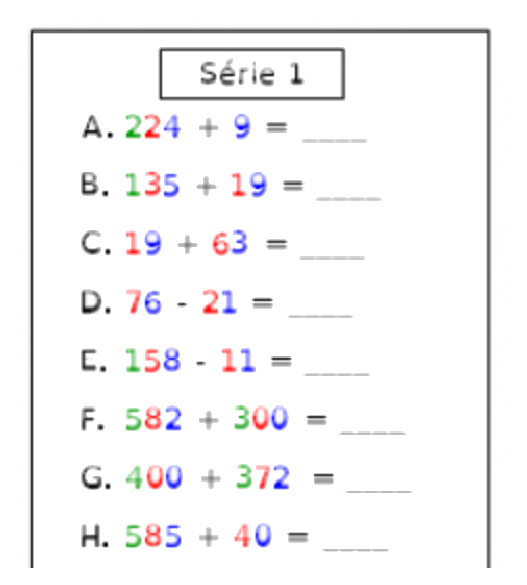
\includegraphics[width=5.5cm]{Nombres_et_calculs_did/Images/Num2_cours_calcul_mental}
   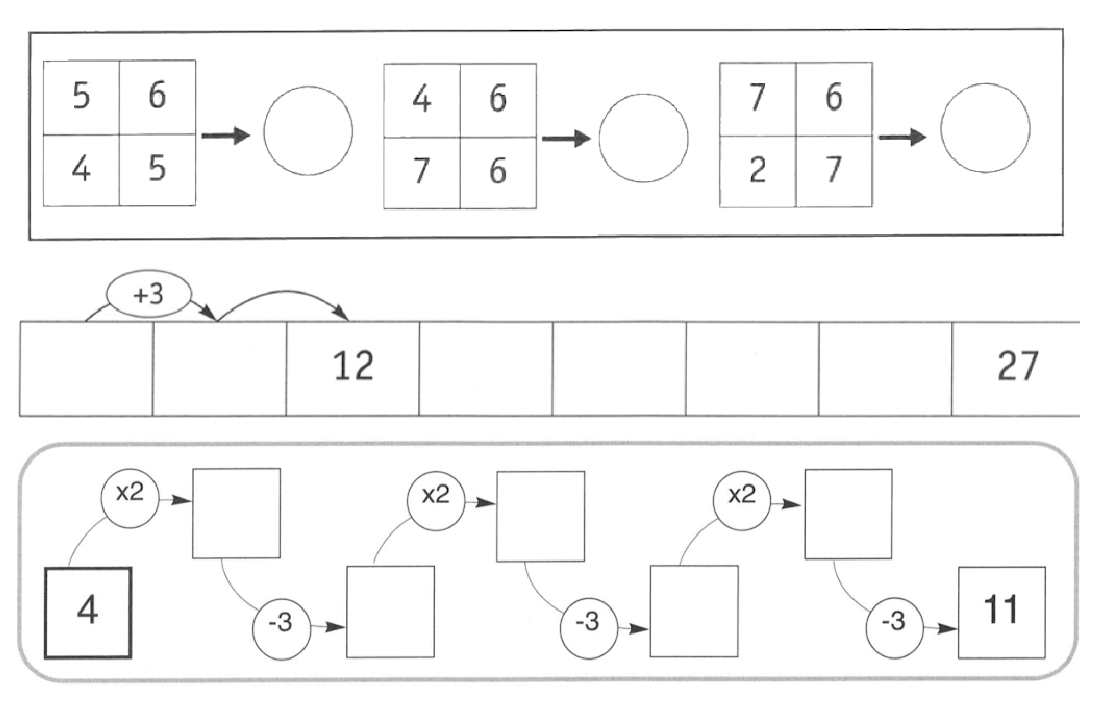
\includegraphics[width=11cm]{Nombres_et_calculs_did/Images/Num2_cours_Boule}
\end{center}


%%%%%%%%%%%%%%%%%%%%%%%
\subsection{Progressivité des apprentissages} 

\begin{description}
   \item[Au cycle 1 :] l’élève apprend à quantifier des collections jusqu’à dix, il les compose et les décompose par manipulations effectives puis mentales. \\
   Il apprend à dire combien il faut ajouter ou enlever pour obtenir des quantités ne dépassant pas dix et parle des nombres à l’aide de leur décomposition. \\
   Ces premiers travaux, nécessaires pour la construction de la notion de nombre, sont aussi les premiers apprentissages du calcul.
   
   \item[Au cycle 2 :] les élèves établissent puis doivent progressivement mémoriser des faits numériques et des procédures. \\
      {\bf Au CP}, les élèves apprennent en P1 les compléments à 10 et les décomposition additives pour des nombres inférieurs à 10. \\
      En P2, ils apprennent les doubles des nombres inférieurs à 10 et les moitiés des nombres inférieurs à 20. \\
      En fin d'année, les tables d'additions sont censées être mémorisées. \\
         Concernant les procédures, ils mobilisent tout au long de l'année la propriété de commutativité de l'addition : \og $3+6$, c'est pareil que $6+3$ \fg. \\
      {\bf Au CE1}, ils apprennent les compléments à la dizaine et à la centaine supérieure, puis les doubles et moitiés d'usage courant. \\
         La multiplication par 10, ainsi que les tables de 3, 4 et 5 sont vues à partir de la P3. \\
         Sur cette période, la commutativité de la multiplication est introduite : \og $3\times5$, c’est pareil que $5\times3$ \fg, ainsi que l'associativité : \og $3\times5\times2$, c’est pareil que $3\times10$ \fg{} et la distributivité sur l'addition sur des cas très simples : \og $12\times5 =10\times5+2\times5$ \fg. \\
      {\bf Au CE2}, il apprennent les compléments à 1 000, puis la multiplication par 10 et 1 000, ainsi que les tables de 6 à 9. La distributivité sur la soustraction est mobilisée sur des cas simples : \og $5\times18 =5\times20-5\times2$ \fg. \\
         À partir de la P3, ils développent des procédures concernant la division euclidienne de nombres comme 10, 25, 50 et 100 par un nombre à 1 chiffre à l'oral : \og 92 divisé par 9, il y a 10 fois 9 et il reste 2 \fg.
         
   \item [Au cycle 3 :] tout au long du cycle, la pratique régulière du calcul conforte et consolide la mémorisation des tables de multiplication jusqu’à 9. \\
      {\bf Au CM1}, les élèves apprennent les quatre premiers multiples de 25 et 50. \\
         À partir de la P3, ils apprennent à multiplier et à diviser par 10 des nombres décimaux et recherchent le complément au nombre entier supérieur. Il apprennent également les critères de divisibilité par 2, 5 et 10. \\
         En fin d'année, ils multiplient par 1 000 un nombre décimal. \\
         Les propriétés des opérations sont stabilisées tout au long de l'année. \\
      {\bf Au CM2}, ils apprennent très vite à diviser un nombre décimal par 100. \\
         En P3, ils multiplient un nombre décimal par 5 et 50, puis apprennent les critères de divisibilité par 3 et 9. \\
         Les propriétés des opérations sont approfondies sur des calculs plus complexes par la nature des nombres, leur taille ou leur nombre.
\end{description}

\medskip


\begin{remarque}
   on peut facilement retrouver le résultat de la table des 9 \\
   \begin{minipage}{10.5cm}
   avec nos mains. Par exemple, calculons $8\times9$ :
  \begin{itemize}
         \item placer les faces des mains devant soi, abaisser le 8\up{e} doigt ;
         \item les doigts à gauche représentent le nombre de dizaines ;
         \item les doigts à droite représentent le nombre d'unités.
      \end{itemize}
      donc $8\times9 =72$.
      \end{minipage}
      \begin{minipage}{2cm}
         \rput(2.5,0.6){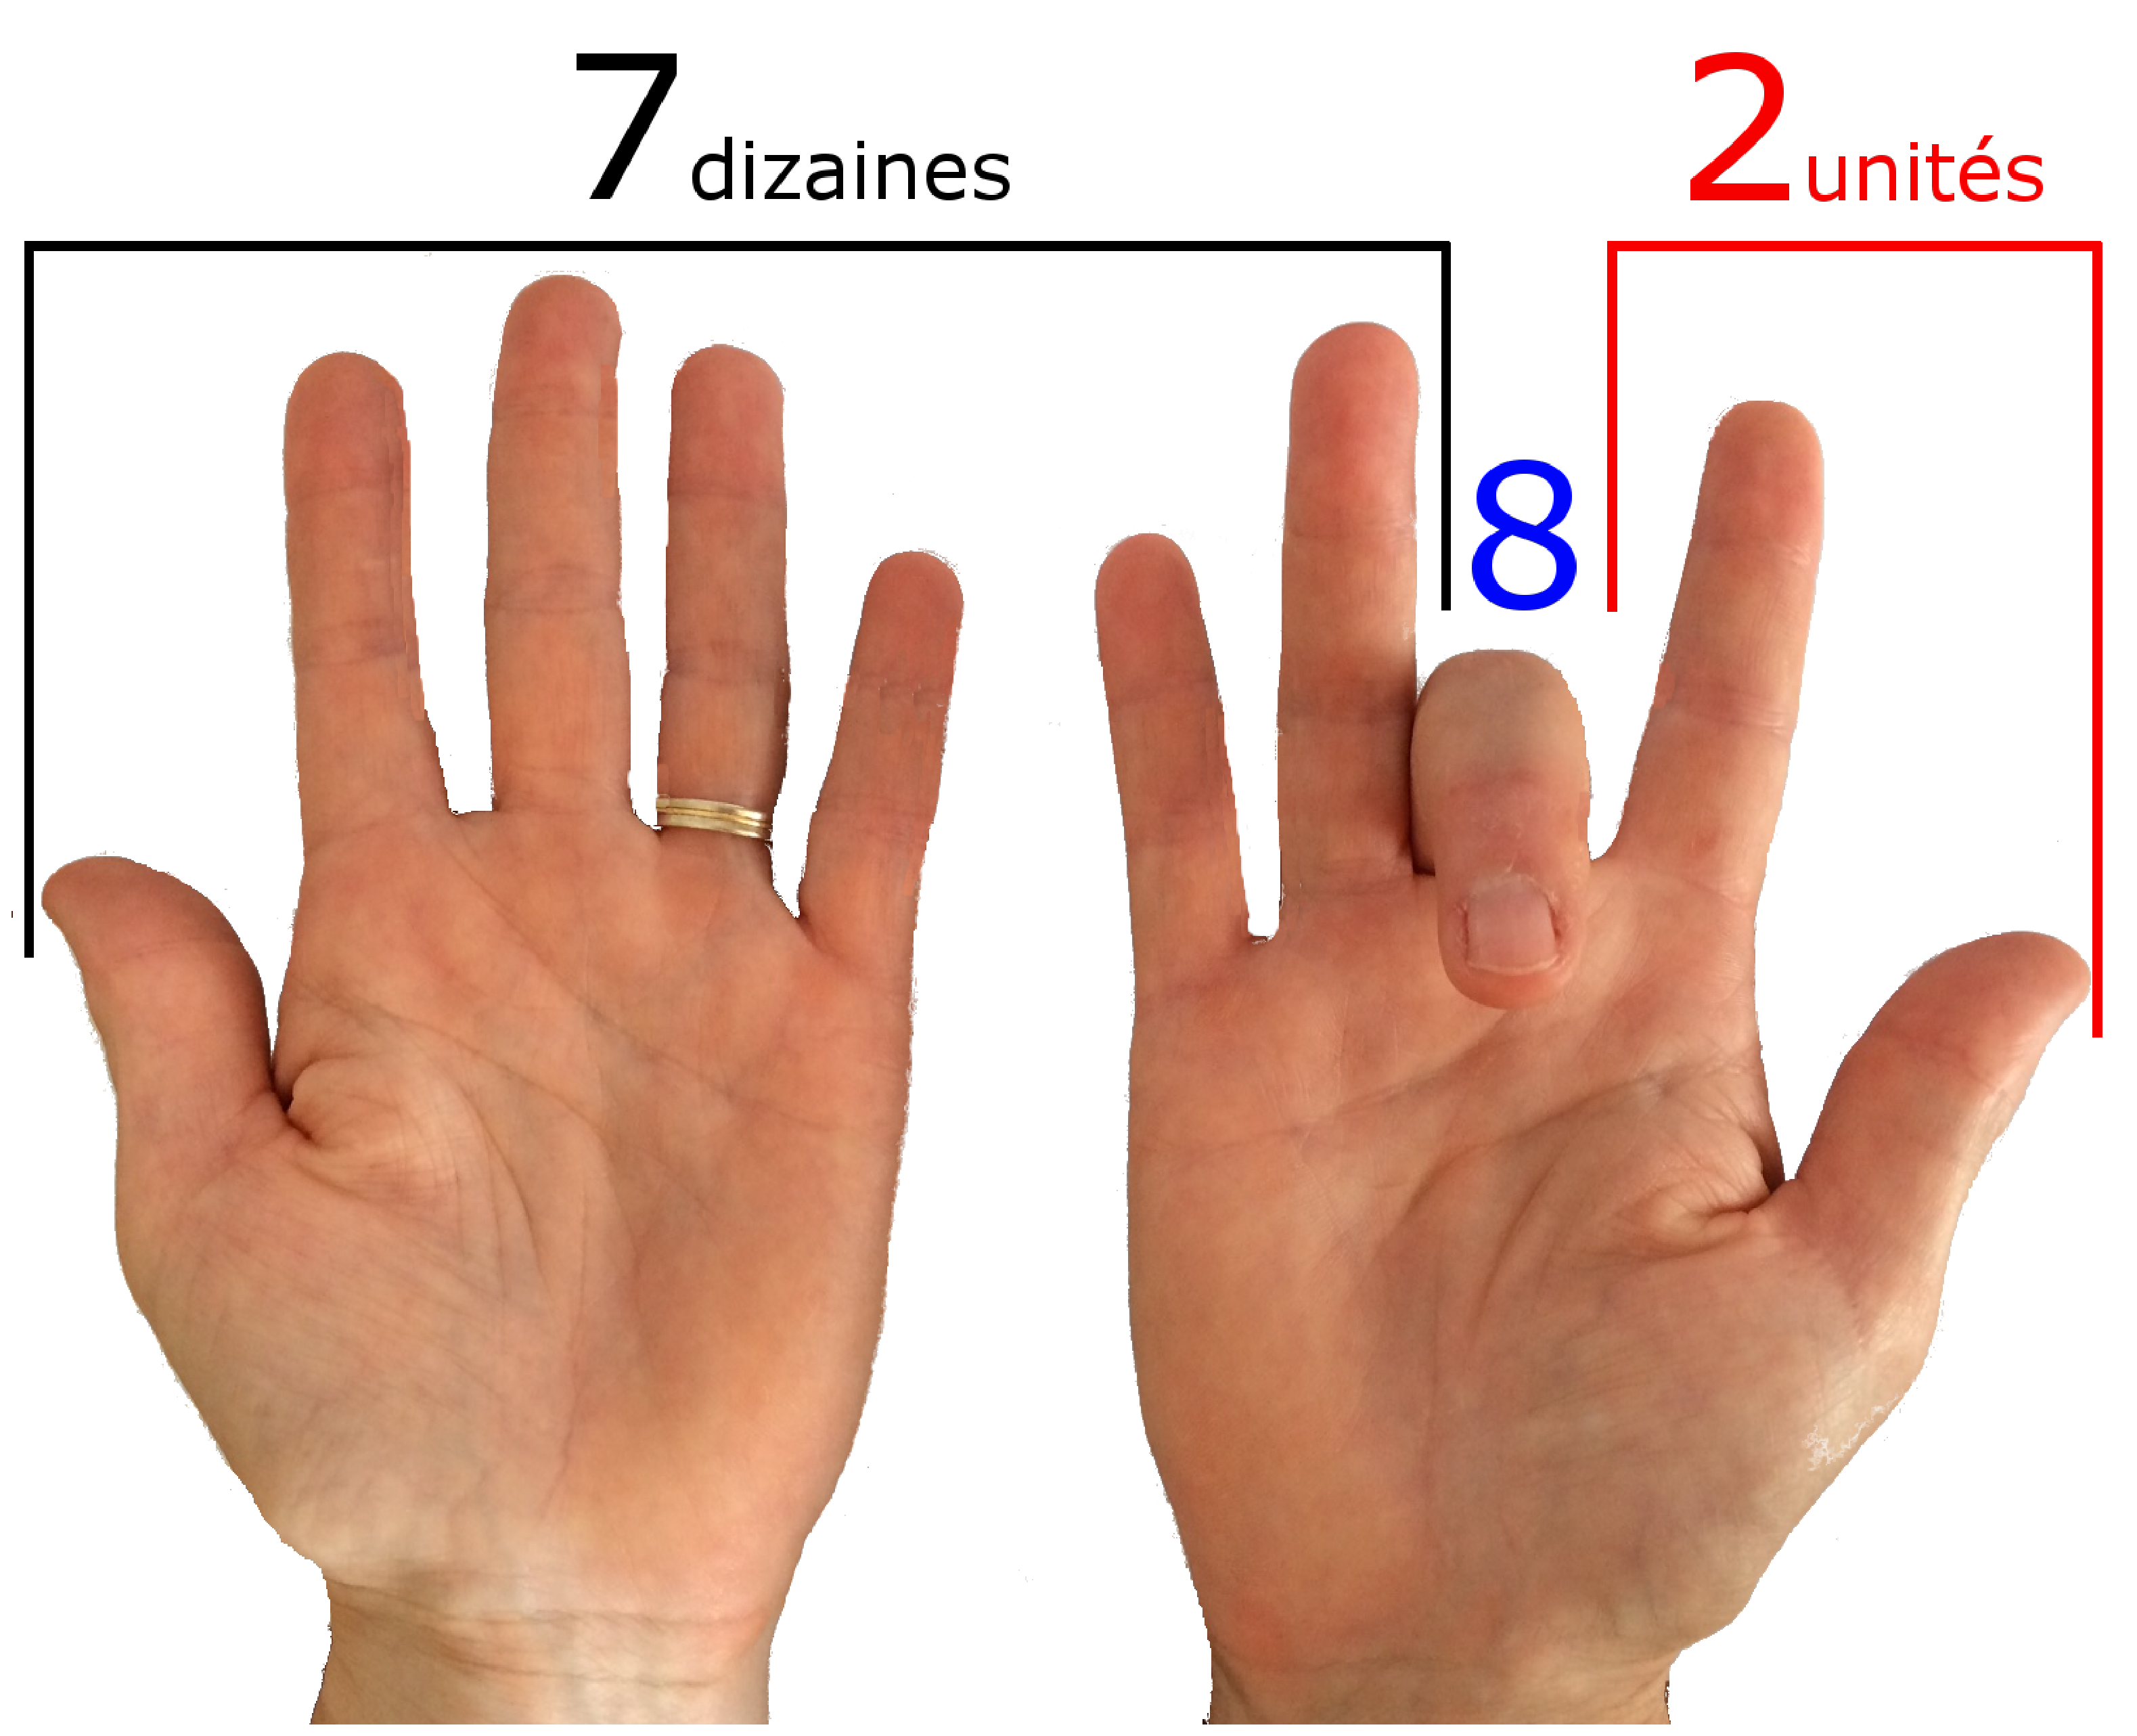
\includegraphics[width=3cm]{Nombres_et_calculs_did/Images/Num2_cours_mains}}
      \end{minipage}
   \end{remarque}
      
\pagebreak


%%%%%%%%%%%%%%%%
\section{Le calcul posé en ligne}
%%%%%%%%%%%%%%%%

D'après le document Éduscol : \og Le calcul en ligne au cycle 2 \fg{} [édu2], le calcul en ligne est une modalité de calcul écrit ou partiellement écrit. Il se distingue à la fois : \\
   -- du calcul mental, en donnant la possibilité à chaque élève, s’il en ressent le besoin, d’écrire des étapes de calculs intermédiaires qui seraient trop lourdes à garder en mémoire ; \\
   -- du calcul posé en colonnes, dans le sens où il ne consiste pas en la mise en œuvre d’un algorithme. \medskip
   
   Le calcul en ligne repose sur la compréhension de la notion de nombre, du principe de la numération décimale de position et des propriétés des opérations. En calcul en ligne, les étapes écrites utiles pour l’élève peuvent, dans un premier temps, se présenter sous différentes formes : calculs séparés, arbres de calcul, écritures utilisant des mots ou des flèches, ou tout autre écrit qui accompagne la démarche de l’élève.


%%%%%%%%%%%%%%%%%%%
\subsection{Règles du calcul en ligne}

L'oralisation du calcul en ligne implique un minimum de connaissances au niveau du vocabulaire.
\begin{center}
   {\hautab{1.5}
   \begin{Ltableau}{0.878\linewidth}{4}{C{2}|C{2.5}|C{2}|C{6.55}}
      \hline
      Signe & opération & résultat & exemple \\
      \hline
     plus : $+$ & addition & somme & $3+4 =7$ : la somme de 3 et de 4 est 7 \\
      \hline
      moins : $-$ & soustraction & différence & $7-3 =4$ : la différence entre 7 et 3 est 4 \\
      \hline
      multiplié : $\times$ & multiplication & produit & $8\times2 =16$ : le produit de 8 et de 2 est 16 \\
      \hline
      divisé : $\div$ & division & quotient & $16\div2 =8$ : le quotient de 16 par 2 est 8 \\
      \hline
   \end{Ltableau}}
\end{center}
   
Il est important, dès le début du cycle 2, de travailler en même temps l'addition et la soustraction, afin de montrer le lien fort qui les unit.
 
\begin{center}
   {\psset{unit=0.8}
   \begin{pspicture}(0,0.5)(12,6)
      \psellipse[linecolor=A1](1.8,3)(1.5,1.25)
      \psdots[linewidth=2mm,linecolor=A1](1.1,2.5)(1.5,3.5)(2.5,2.8)
      \psline[linecolor=A1](1.4,4.2)(1,5)
      \rput(0.8,5.3){\textcolor{A1}{\large 3}}
      \psellipse[linecolor=B1](5.5,3)(2,1.5)
      \psdots[linewidth=2mm,linecolor=B1](4.3,3)(5.6,3.6)(6,2.5)(7,3)
      \psline[linecolor=B1](6,4.45)(6.3,5.3)
      \rput(6.4,5.6){\textcolor{B1}{\large 4}}
      \psellipse(4,3)(4,2)
      \psline(4,5)(4,5.7)
      \rput(4,6){\large 7}
      \rput(11,4.5){$3+4 =7$}
      \rput(11,3.5){$4+3 =7$}
      \rput(11,2.5){$7-3 =4$}
      \rput(11,1.5){$7-4 =3$}
   \end{pspicture}}
\end{center}
   
Le {\bf statut du signe \og = \fg{}} est souvent interprété comme un signe permettant l’affichage du résultat après exécution d’un calcul alors qu'il caractérise l'équivalence entre le membre écrit à sa droite et celui écrit à sa gauche.
  
\begin{exemple*1}
   {\small
   J'avais 12 billes en arrivant à l'école, j'en ai gagné 10 à la récréation et encore 2 autres à la pause méridienne. J'ai donc maintenant 24 billes. \\
   L'élève aura tendance à écrire $12+10 =22+2 =24$.}
\end{exemple*1} \medskip

Cette écriture du calcul n'est pas correcte d'un point de vue mathématique. Elle ne doit pas être proposée au tableau, mais ne doit pas non plus être sanctionnée ; la démarche de l’élève est correcte, c’est l’utilisation du symbole de l’égalité qui ne l’est pas, il faut donc lui expliquer et éviter de laisser s'installer de mauvaises habitudes. \bigskip

Afin de transiter vers le calcul en colonnes, les élèves apprennent à ajouter des nombres en ligne, en les décomposant en dizaines-unités, puis en ajoutant séparément les dizaines et les unités avant de reconstituer le résultat. 
   
\begin{exemple*1}
   {\small
   $65 + 17 = (60 + 5) + (10 + 7) = (60 + 10) + (5 + 7) = 70 + 12 = 82$. \\
    Pour matérialiser cette façon de calculer, on peut avoir recours à un {\bf arbre de calcul}. \\ [1mm]
  \psset{nodesep=3pt,linecolor=A1}
     \hspace*{3cm} $65+17 = \quad \rnode{a}{60} \quad + \quad \rnode{b}{5} \quad  + \quad \rnode{c}{10} \quad  + \quad \rnode{d}{7}$ \\ [5mm]  
     \hspace*{3cm} $\phantom{65+17} = \quad \rnode{e}{60} \quad + \quad\rnode{f}{10} \quad + \quad \rnode{g}{5} \quad + \quad \rnode{h}{7}$
     \ncline{a}{e} \ncline{c}{f} \ncline{b}{g} \ncline{d}{h} \\ [5mm]
     \hspace*{3cm} $\phantom{65+17} = \qquad \, \quad \rnode{i}{70} \qquad \quad + \qquad \quad \rnode{j}{12}$
     \ncline{e}{i} \ncline{f}{i} \ncline{g}{j} \ncline{h}{j} \\ [5mm] 
     \hspace*{3cm} $\phantom{65+17} = \qquad \qquad \qquad \quad \, \rnode{k}{82}$
     \ncline{i}{k} \ncline{j}{k}} \\ [-3mm]
\end{exemple*1}    

\ \\

Les premières situations multiplicatives consistent généralement à donner des activités de dénombrement de collections rangées par paquets équipotents ou de manière rectangulaire. \\
Ainsi, les élèves découvrent l'{\bf écriture multiplicative} comme représentant le nombre d'objets d'une collection rangée en lignes et colonnes. Il s'agit de l'addition itérée. Cela permet notamment d'installer la {\bf commutativité de la multiplication}.

\begin{exemple*1}
   {\small
   \begin{pspicture}(-1,0)(13,1)
      \multido{\n=0+0.75}{5}{\rput(\n,0){\Large$\bigstar$}}
      \multido{\n=4.50+0.75}{5}{\rput(\n,0){\Large$\bigstar$}}
      \multido{\n=9+0.75}{5}{\rput(\n,0){\Large$\bigstar$}}
   \end{pspicture} \\
   \begin{pspicture}(-5,-0.75)(4,1)
      \multido{\n=0+0.75}{5}{\multido{\r=0+0.75}{3}{\rput(\n,\r){\Large\textcolor{A1}{$\bigstar$}}}}
   \end{pspicture} 
   \begin{pspicture}(-2,0)(2,4)
      \multido{\n=0+0.75}{3}{\multido{\r=0+0.75}{5}{\rput(\n,\r){\Large\textcolor{B1}{$\bigstar$}}}}
   \end{pspicture} \\ [3mm]
   On a les représentations de $5+5+5 =3\times5 =5\times3$.}
\end{exemple*1}

\bigskip


%%%%%%%%%%%%%%%%%%%%%%%
\subsection{Progressivité des apprentissages} 

Les connaissances et compétences mises en œuvre pour le calcul en ligne sont les mêmes que pour le calcul mental, le support de l’écrit permettant d’alléger la mémoire de travail et ainsi de traiter des calculs portant sur un registre numérique étendu.

%\subsection{Des précisions concernant les parenthèses dans le calcul en ligne}
%%%%%%%%%%%%%%%%%%%%%%
%
%D'après les documents éduscol : \og {\it Le calcul en ligne au cycle 2} \fg{} et \og {\it Le calcul en ligne au cycle 3} \fg.
%
%L’apprentissage de l’utilisation des parenthèses débute au cycle 3. Les règles des priorités mathématiques imposent de commencer, dans un calcul en ligne, par les multiplications et les divisions (dans n'importe quel ordre), puis les additions et soustractions. \medskip
%
%On peut, de façon générale, distinguer deux usages des parenthèses dans les calculs : \\
%$\bullet$ une indication de la façon dont on va organiser les calculs, même si du point de vue mathématique le code des priorités opératoires est clair.
%\begin{exemple*1}
%   $26\times5 = (13\times2)\times5 = 13\times(2\times5) = 13\times10 = 130$. \\
%   Il s'agit de l'{\bf associativité de la multiplication}.
%\end{exemple*1}
%
%\bigskip
%
%$\bullet$ un impératif pour indiquer que le calcul ne doit pas se faire selon le code établi des priorités opératoires.
%\begin{exemple*1}
%   $(5 + 8) \times 7 = 13 \times 7 = 91$.
%\end{exemple*1}
%
%\bigskip
%
%Au cycle 2, la maîtrise du code des priorités opératoires n’est absolument pas un objectif. Il faut tout d’abord que les élèves s’approprient le sens de chacune des opérations. Lorsqu’ils doivent organiser des calculs mobilisant successivement deux opérations éventuellement identiques, l’utilisation de plusieurs lignes est à privilégier. \\
%
%{\bf Quelques rappels concernant l’utilisation de parenthèses.} \\
%$\bullet$ Dans un calcul, l’écriture des parenthèses peut ou non être évitée.
%\begin{exemple*1}
%\ \\[1mm]
%\begin{tabular}{p{7cm}|p{7.8cm}}
%   $15 \times 6 = (3 \times 5) \times 6 = 3 \times (5 \times 6) = 3 \times 30 = 90$.
%   &
%   $15 \times 6 = (10 + 5) \times 6 = 10\times6+5\times6 =60 + 30 = 90$. \\
%   Les parenthèses apparaissent comme des boites qui indiquent les transformations effectuées lors du calcul, leur présence sert à communiquer, à rendre plus visible ce qui est fait; sur le plan mathématique, les parenthèses pourraient être retirées.
%   &
%   Les parenthèses servent à mettre en lumière la transformation de 15 en $10 + 5$ et sont mathématiquement indispensables. En effet, si on les retire, on obtient : $10 + 5 \times 6 =10+30 =40$. \\
%\end{tabular}
%\end{exemple*1}
%
%\bigskip
%
%$\bullet$ Le calcul \og $6 \times 10 + 6 \times 5$ \fg{} ne nécessite pas de parenthèses dès lors que les règles de priorité sont connues ; on pourra toutefois préférer écrire \og $(6 \times 10) + (6 \times 5)$ \fg{} pour bien spécifier les calculs à faire en premier.


\newpage


%%%%%%%%%%%%%%%%%%%%
\section{Résolution de problèmes} %%%
%%%%%%%%%%%%%%%%%%%%

%%%%%%%%%%%%%%%%%%%%
\subsection{Qu'est-ce qu'un problème ?} 


\og Il y a des problèmes lorsqu’on peut apporter des réponses par des raisonnements. Il faut qu’il y ait quelque chose à chercher et qu’il ne soit pas possible d’utiliser la mémoire seule. \fg{} {\it Guy Brousseau}. \\ [1mm]
\og Un problème est généralement défini comme une situation initiale avec un but à atteindre, demandant au sujet d’élaborer une suite d'actions ou d'opérations pour atteindre ce but. \fg{} {\it Jean Brun, Dominique Valentin}.

Le même énoncé peut constituer un problème, ou un exercice selon le niveau auquel on le propose :
\begin{exemple*1}
   {\small
   J’ai 38 billes et j’en ai gagné 23 à la récré. Combien avais-je de billes ce matin? \\
   Au CP, il s'agit d'un problème puisqu'il va falloir trouver une solution personnelle, pour laquelle la technique experte n'est pas connue. Au CM1, il s'agit d'un exercice.}
\end{exemple*1}

\medskip

Aujourd’hui, il y a un consensus sur la place centrale que doit occuper la résolution de problèmes dans l’enseignement des mathématiques à l’école primaire comme au collège. Dans le rapport dirigé par {\it Cédric Villani} et {\it Charles Torossian} datant de février 2018 : \href{https://www.education.gouv.fr/21-mesures-pour-l-enseignement-des-mathematiques-3242}{\blue\og 21 mesures pour l'enseignement des mathématiques \fg} [vil18], la cinquième des 21 mesures concerne les étapes d'apprentissage : 
\og Dès le plus jeune âge mettre en oeuvre un apprentissage des mathématiques fondé sur : \\
   -- la manipulation et l’expérimentation ; \\
   -- la verbalisation ; \\
   -- l’abstraction. \fg

La résolution de problèmes permet de mettre en \oe uvre ce cinquième fondement, selon le schéma suivant, par exemple :

\begin{pspicture}(0.5,4.5)(16,15.5)
   \psline[linewidth=1mm]{->}(10,15.5)(10,4.2)
   \rput(1.5,14){\it Agir}
   \rput(6.5,14){\parbox{7cm}{Faire, manipuler, essayer, recommencer \\ Prendre des initiative \\ Décider}}
   \rput(14,15.3){\bf Manipuler, expérimenter}
   \rput(14,14){
\includegraphics[width=4cm]{Nombres_et_calculs_did/Images/Num2_cours_manipuler}} %%%
   \rput(1.5,11.5){\it Réussir}
   \rput(6.5,11.5){\parbox{7cm}{Aller au bout d'une démarche \\ Prendre plaisir \\ Être vu par l'adulte en train de réussir}}
   \rput(14,11.7){
\includegraphics[width=2.5cm]{Nombres_et_calculs_did/Images/Num2_cours_reussir}} %%%
   \rput(1.5,8.8){\it Comprendre}
   \rput(6.5,8.8){\parbox{7cm}{Pourquoi, comment on a réussi \\ Mettre des mots sur ses réussites}}
   \rput(14,10.2){\bf verbalier}
   \rput(14,9){
\includegraphics[width=3.5cm]{Nombres_et_calculs_did/Images/Num2_cours_verbaliser}} %%%
   \rput(1.5,6){\it Généraliser}
   \rput(6.5,6){\parbox{7cm}{Conjecturer, représenter de manière générale \\ Passer d'une représentation concrète\\à imagée à abstraite, utiliser des symboles}}
   \rput(14,7.3){\bf Abstraire}
   \rput(14.1,6.15){
\includegraphics[width=8cm]{Nombres_et_calculs_did/Images/Num2_cours_abstraction}} %%%
\end{pspicture}


%%%%%%%%%%%%%%%%%%%%%%
\subsection{Catégorisation des problèmes} 

Le guide \og \href{https://eduscol.education.fr/document/32206/download?attachment}{\blue La résolution de problèmes mathématiques au cours moyen} \fg{} [men22], édité en 2022 par le ministère de l'éducation nationale, fait émerger un exemple de catégorisation de problèmes en trois catégories principales, en rapport avec les travaux de {\it Catherine Houdement} et résumées pas le schéma suivant :
   \begin{center}
      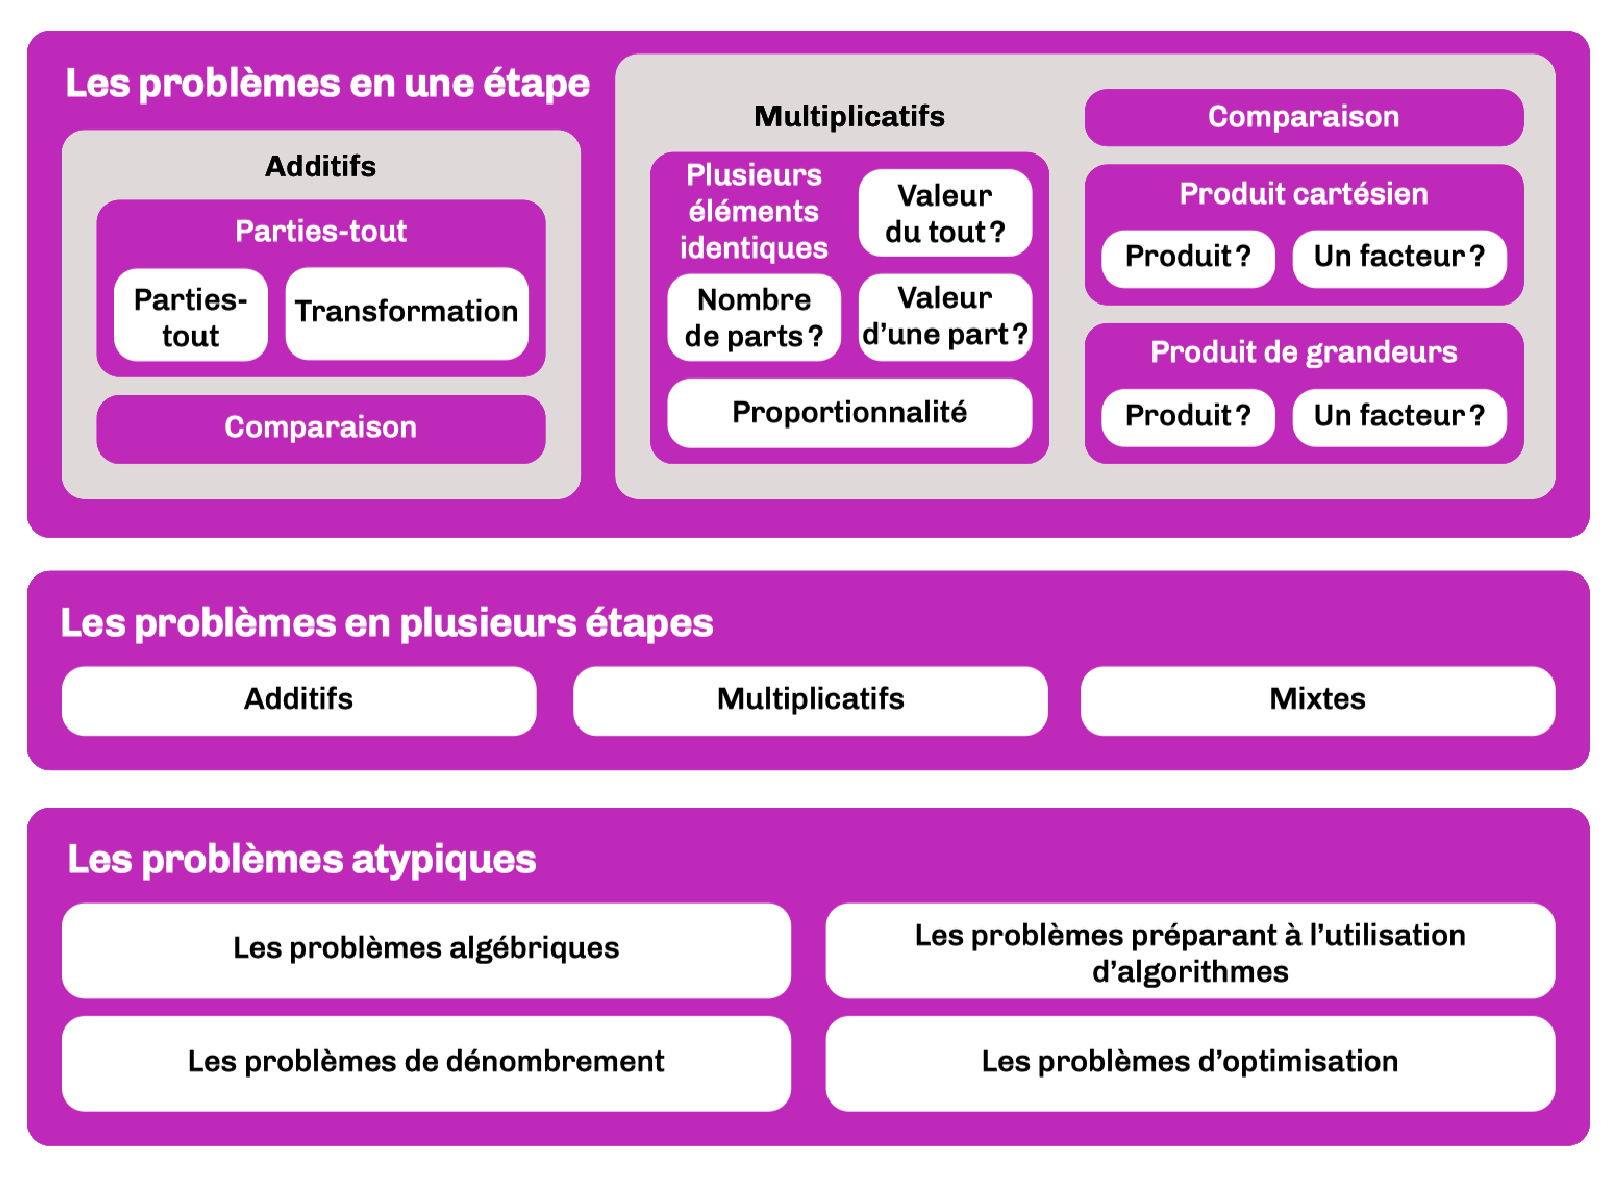
\includegraphics[width=13cm]{Nombres_et_calculs_did/Images/Num2_cours_tableau_problemes}
   \end{center}

   -- {\bf Les problèmes en une étape :} ce sont des problèmes qui vont se traiter en effectuant une unique opération. \\
   Le travail du CM va être de construire des modélisations permettant de résoudre ces types de problèmes de manière quasi-automatisée.
      \begin{exemple*1}
         {\it Catherine Houdement} propose quatre problèmes en une étape :
         {\small
         \begin{enumerate}
            \item Un massif de fleurs est formé de 60 tulipes rouges et de 15 tulipes noires. Combien y a-t-il de tulipes dans ce massif ?
            \item Un massif est formé de 60 rangées, toutes de 15 tulipes. Combien y a-t-il de tulipes dans ce massif ?
            \item Un massif de 60 fleurs est composé de tulipes et de 15 jonquilles. Combien y a-t-il de tulipes dans ce massif ?
            \item 60 tulipes sont disposées en 15 massifs tous identiques. Combien y a-t-il de tulipes dans un massif ? \\ [-8mm]
         \end{enumerate}}
      \end{exemple*1} \medskip
      Ces problèmes ont des points communs : on y parle de massifs de fleurs et de tulipes et ils contiennent, tous, les nombres 60 et 15. \\
      Toutefois, la résolution se fera par des opérations différente : dans nos exemples, les problèmes 1) et 3) sont des problèmes additifs de parties-tout (le premier se résout à l'aide d'une addition, le troisième grâce à une soustraction). \\
      Les problèmes 2) et 4) sont des problèmes multiplicatifs à plusieurs éléments identiques (le deuxième fait appel à une multiplication et le quatrième à une division). \\
      On trouvera dans le guide de multiples exemples expliquant les autres sous-types de problème en une étape. \\
      
   -- {\bf Les problèmes en plusieurs étapes :} ce sont des problèmes qui vont se traiter comme une succession de problèmes en une étape qui vont permettre d’aboutir à la solution recherchée. \\
      La difficulté des problèmes en plusieurs étapes n’est pas la simple somme des difficultés des sous-problèmes en une étape qui les composent. Il faut également ajouter la difficulté de la mise en relation de ces différents sous-problèmes élémentaires. La résolution de problèmes en plusieurs étapes va permettre de renforcer les habiletés de résolution de problèmes en une étape.
      \begin{exemple*1}
         {\small
         \begin{enumerate}
            \item Une bouteille de jus de pomme coûte 1,87 zed. Une bouteille de jus d’orange coûte 3,29 zeds. Julien a 4~zeds. Combien de zeds Julien doit-il avoir en plus pour acheter les deux bouteilles ?
            \item Un supermarché a commandé une palette de barquettes de fraises. La palette est constituée de 12 étages de cageots et il y a 5 cageots sur chaque étage. Dans chaque cageot, il y a 12 barquettes de 400 g de fraises. Quelle masse de fraises y a-t-il sur la palette ?
            \item Lydia achète 5 billets de cinéma à 7,30 \euro. Elle donne un billet de 50 \euro{} à l’employé de caisse. Combien celui-ci va-t-il lui rendre ? \\ [-10mm]
         \end{enumerate}}
      \end{exemple*1} \medskip
      
      Ici, le premier exemple est un problème en deux étapes dans le domaine additif, le deuxième est un problème en trois étapes dans le domaine multiplicatif et le troisième un problème mixte en deux étapes. \\
      
   -- {\bf les problèmes atypiques :} ce sont des problèmes verbaux à données numériques qui ne rentrent pas dans les catégories des problèmes en une ou plusieurs étapes mentionnées précédemment. \\
      Cette catégorie est moins centrale, mais importante à mettre en place au CM : la résolution des problèmes atypiques doit permettre aux élèves de développer des compétences transversales comme l’autonomie, la prise de décisions, la créativité\dots{} et de rencontrer un certain nombre de stratégies et de types de raisonnements.
      \begin{exemple*1}
         {\small
         \begin{enumerate}
            \item Dans une ferme, il y a des lapins et des poules. Pour faire chercher le nombre de poules et de lapins à son frère, Cindy lui dit qu’il y a 114 pattes et 40 têtes. Combien y a-t-il de poules et combien y a-t-il de lapins dans la ferme ?
            \item Combien peux-tu écrire de nombres à deux chiffres en utilisant uniquement les chiffres 2, 3, 4 et 5 ? Le même chiffre ne peut être utilisé qu’une fois.
            \item Un rectangle a ses côtés qui ont pour longueur des nombres entiers de centimètres. Son aire est de \ucmc{100}. Trouve toutes les dimensions possibles pour ce rectangle.
            \item Parmi les rectangles qui ont leurs côtés mesurant un nombre entier de centimètres et dont le périmètre est \ucm{20}, détermine celui qui a la plus grande aire. \\ [-10mm]
         \end{enumerate}
         }
      \end{exemple*1} \medskip
      Le premier problème est considéré comme algébrique, car il pourra être résolu au C4 grâce à l'algèbre (résolution par une ou plusieurs équations). Au C3, l'élève pourra procéder par essais et ajustements en choisissant des valeurs arbitraires, en effectuant les calculs et en ajustant jusqu'à ce qu'une valeur convienne ; par un traitement pré-algébrique en modélisant la situation, par exemple, par une représentation en barres pour en isoler l'inconnue ; ou encore par un raisonnement déductif en réfléchissant aux valeurs choisies afin d'être plus efficace. \\
      Le deuxième exemple est un problème de dénombrement qui demande une certaine organisation. L'élève pourra le résoudre, par exemple, à l'aide d'un tableau ou d'un arbre. \\
      Le troisième exemple fait partie des problèmes préparant à l’utilisation d’algorithmes et qui consistent à rechercher des solutions vérifiant certaines conditions parmi un ensemble de cas possibles. Ici, il doit chercher les couples de nombres entiers strictement positifs dont le produit est 100. De tels problèmes pourront se traiter dans le second degré en écrivant un programme permettant de balayer tous les cas possibles. \\
      Enfin, le dernier problème est un problème d'optimisation et consiste à trouver la meilleure solution possible tout en respectant un certain nombre de contraintes. 
      

D'autres catégorisations existent, basées davantage sur les types de connaissances et compétences à acquérir.  

{\hautab{1.5}
\small
\begin{CLtableau}{\linewidth}{4}{c}
   \hline
   & Contexte & Objectifs & \it Exemples \\
   \hline
   \parbox{2mm}{\rotatebox{90}{Situation-problème}}
   &
   \parbox{5cm}{\rule{0mm}{4mm}Situation où le problème permet aux élèves d’acquérir des connaissances nouvelles. \newline
   Deux types de problèmes : ceux pour lesquels les élèves disposent de connaissances pas optimales pour le traiter ; ceux pour lesquels les connaissances initiales des élèves ne permettent pas de résoudre le problème directement. \medskip}
   &
   \parbox{5cm}{$\bullet$ Prendre conscience de ce qu'est un problème \newline
      $\bullet$ Emettre des hypothèses \newline
      $\bullet$ Remettre en cause le savoir antérieur \newline
      $\bullet$ Induire un comportement de recherche \newline
      $\bullet$ Construire de nouveaux savoirs}
   &
   \parbox{5cm}{\it C1 : une boite d'\oe ufs représente un bus. Certaines places sont prises par des bonhommes. Aller en une seule fois chercher le nombre de bonhommes nécessaire pour remplir le bus. \newline \newline
   \it CE2 : je veux répartir 756 \oe ufs dans des boîtes de 12 \oe ufs. Combien me faut-il de boîtes ?} \\
   \hline
   \parbox{2mm}{\rotatebox{90}{Réinvestissement}}
   &
   \parbox{5cm}{\rule{0mm}{6mm}Problème visant le transfert et l’utilisation de connaissances antérieures : l'acquisition de connaissances dans un contexte particulier ne suffit pas à leur ancrage. On propose donc un problème utilisant ces connaissances dans un autre contexte. Ce problème peut être un problème complexe nécessitant la mobilisation de plusieurs connaissances mathématiques. \medskip}
   &
   \parbox{5cm}{$\bullet$ Reconnaitre, identifier et interpréter des données \newline
   $\bullet$ Rechercher des informations sur différentes supports \newline
   $\bullet$ Mobiliser des connaissances construites précédemment dans un contexte différent à bon escient et de façon autonome \newline
   $\bullet$ Contextualiser, décontextualiser, recontextualiser}
   &
   \parbox{5cm}{\it C2 : Tom a gagné 3 paquets de Pokémon. il y a 5 cartes par paquets. Combine Tom a-t-il gagné de cartes Pokemon ? \newline \newline
   \it CM1/CM2 : je veux répartir 756 \oe ufs dans des boîtes de 12 \oe ufs. Combien me faut-il de boîtes ?} \\  
   \hline
   \parbox{2mm}{\rotatebox{90}{Problème ouvert}}
   &
   \parbox{5cm}{Problème destiné à mettre l’élève en situation de recherche et développer des compétences d’ordre méthodologique nécessaires pour résoudre des situations problèmes. Pas de démarche préalablement explorée. \newline \newline
   \href{https://edu1d.ac-toulouse.fr/politique-educative-31/ien31-toulouse-sud/files/2019/05/solutions_-pb_chercher_\%C3\%A9nonc\%C3\%A9s-cycle-2-et-3.pdf}{\blue\it Exemples de problèmes ouverts}}
   &
   \parbox{5cm}{\rule{0mm}{4mm}$\bullet$ Acquérir des attitudes et méthodes favorables à la résolution de problème : hypothèses, imaginer une ou plusieurs solutions, les valider, argumenter, utiliser des connaissances antérieures \newline
   $\bullet$ Gérer les essais et les traces écrites, trier, organiser les informations, organiser sa démarche, prendre des initiatives, oser se tromper \medskip}
   &
   \parbox{5cm}{\it CE1 : je veux répartir 756 \oe ufs dans des boîtes de 12 \oe ufs. Combien me faut-il de boîtes ? \newline \newline
   C3 : on dispose de pièces de 50~c, de 20~c et de 5~c. Peut-on constituer la somme de 5 \euro{} avec exactement 20 pièces ?} \\
   \hline
   \parbox{2mm}{\rotatebox{90}{Tâche complexe}}
   &
   \parbox{5cm}{Problème destiné à permettre l’utilisation conjointe de plusieurs connaissances dans des situations plus complexes. Exige de scinder le problème en sous problèmes, de comparer plusieurs solutions et/ou hypothèses et fait appel à plusieurs connaissances, savoirs et savoir-faire. \newline \newline
   \href{http://www.ac-grenoble.fr/ien.g3/IMG/pdf_Complexe_dernier.pdf}{\blue\it Exemples de tâches complexes}}
   &
   \parbox{5cm}{$\bullet$ Prendre des informations dans différentes supports \newline
   $\bullet$ Trier, organiser les informations \newline
   $\bullet$ Utiliser des connaissances antérieures \newline  
   $\bullet$ Gérer les traces écrites et les essais \newline
   $\bullet$ Produire des résultats intermédiaires}
   &
   \parbox{3cm}{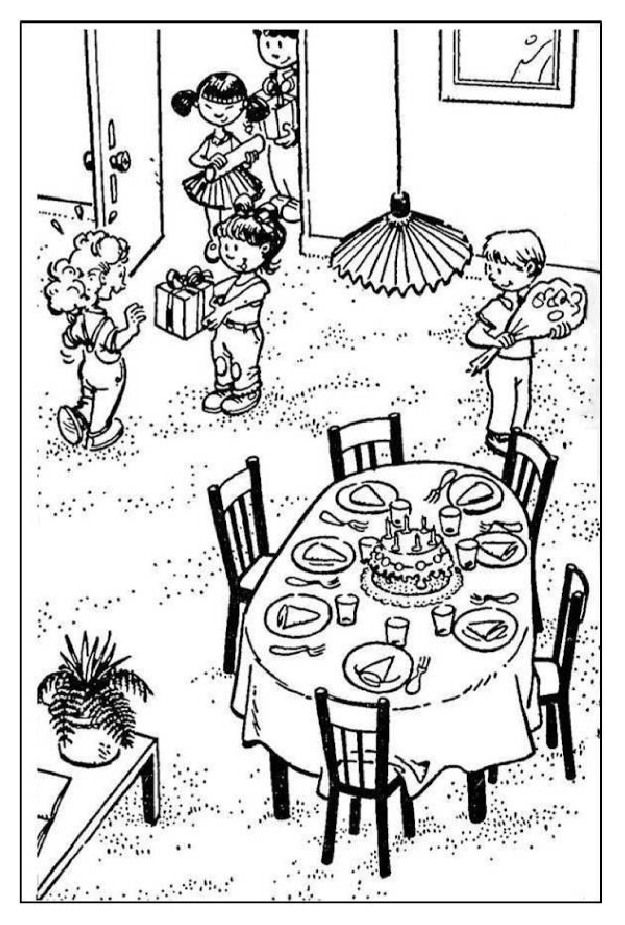
\includegraphics[width=3cm]{Nombres_et_calculs_did/Images/Num2_cours_anniversaire}}
   \parbox{5cm}{\it CP : Anne a préparé un goûter pour fêter son anniversaire. Tous les amis qu’elle a invités sont arrivés. Observe l’image et réponds aux questions. Quel est l'âge d'Anne ? A-t-elle bien préparé sa table ?} \\
   \hline
\end{CLtableau}}

\hfill{\it\small Source : travaux de S. Gano, résolution de problèmes cycle 3, bordas - Documents d'accompagnement des programmes 2002.}


%%%%%%%%%%%%%%%%%%%
\subsection{Les étapes d'un problème}

Dans \og Enseignement et apprentissage des mathématiques.
Que disent les recherches psychopédagogiques \fg{} [ver08], {\it Lieven Verschaffel} et {\it Erik De Corte}  s'expriment ainsi :
\begin{quote}
   \it L’application des mathématiques pour résoudre des problèmes situés dans le monde réel, également appelée modélisation mathématique, peut être conçue comme un processus complexe comprenant plusieurs étapes : la compréhension de la situation décrite ; la construction d’un modèle mathématique qui décrit l’essence de ces éléments et les relations significatives impliquées dans la situation ; l’application du modèle mathématique pour identifier ce qui en découle ; l’interprétation du résultat des calculs afin de parvenir à une solution de la situation pratique qui a donné lieu au modèle mathématique ; l’évaluation du résultat interprété en relation à la situation d’origine ; et la communication des résultats interprétés.
\end{quote}

Le guide de résolution des problèmes en CM retient un modèle assez similaire et synthétique en quatre étapes : comprendre, modéliser, calculer, répondre, résumé par le schéma suivant :
   \begin{center}
      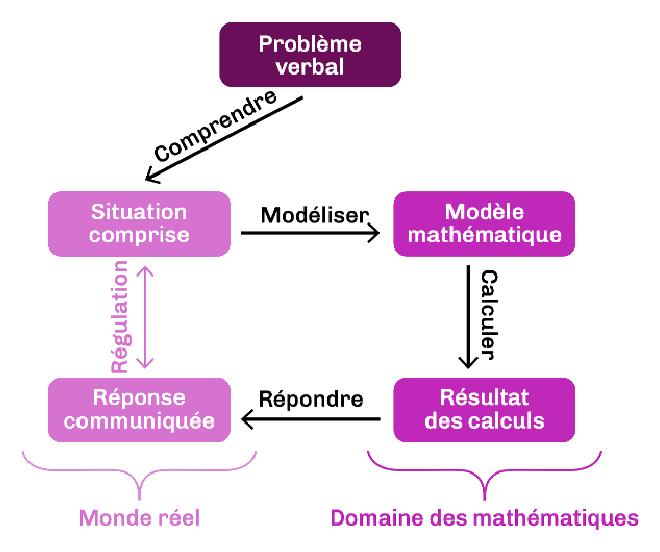
\includegraphics[width=8cm]{Nombres_et_calculs_did/Images/Num2_cours_etapes}
   \end{center}

Nous allons expliciter rapidement ces étapes, à l'aide d'un exemple présent dans le guide :
\begin{exemple*1}
   Marius revient du marché. Il a acheté \ug{750} de fraises, un demi-kilogramme d’abricots et a oublié la masse des kiwis achetés. Le contenu de son panier pèse \ukg{1,650}. \\
   Quelle est la masse des kiwis ?
\end{exemple*1}

{\hautab{1.5}
\begin{longtable}{|p{8cm}|p{8cm}|}
   \hline
   \multicolumn{2}{|>{\columncolor{FondTableaux}}c|}{Comprendre} \\
   \hline
   Un problème est en premier lieu une histoire qu’il va falloir comprendre. \newline
   La compréhension doit être fine alors qu'une compréhension globale et approximative pourrait suffire dans d'autres cadres. \newline
   Il faut également comprendre la question : que cherche-t-on ? quelle est sa nature ?
   &
   Ce que les élèves doivent comprendre et savoir  : \newline
   -- c'est l'historie de Marius qui a fait des achats au marché ; \newline
   -- dans son panier, il y a des fraises, des abricots et des kiwis, dont Marius a oublié la masse ; \newline
   -- il n’y a rien d’autre dans le panier (implicite) ; \newline
   -- les masses s’additionnent pour former la masse du contenu du panier ; \newline
   --  un demi-kilogramme, c'est comme 0,5 kg ou 500 g ; \newline
   -- on cherche la masse des kiwis. \\
   \hline \pagebreak
   \hline
   \multicolumn{2}{|>{\columncolor{FondTableaux}}c|}{Modéliser} \\
   \hline
   La modélisation est le \og processus par lequel l’individu convertit les données des situations réelles en problème mathématique \fg. \newline
   Elle aboutit à déterminer, en s’appuyant sur d’éventuelles représentations (dessins, schémas, tableaux, arbres, etc.), quelles opérations devront être effectuées dans la phase suivante pour répondre à la question posée.
   &
   -- Nous sommes dans un problème à plusieurs étapes du type \og parties-tout \fg ; \newline
   -- une difficulté supplémentaire provient du fait que les unités ne soient pas homogènes ; \newline
   -- la modélisation peut se faire (par exemple) à l'aide d'un schéma en barres : \newline
   \begin{pspicture}(-0.25,0.25)(7.5,2.2)
      \psframe(0,0.25)(7.5,2)
      \psline(0,1)(7.5,1)
      \psline(2.5,1)(2.5,2)
      \psline(5,1)(5,2)
      \rput(1.25,1.7){Fraises}
      \rput(1.25,1.3){\ug{750}}
      \rput(3.75,1.7){Abricots}
      \rput(3.75,1.3){1/2 kg}
      \rput(6.25,1.7){Kiwis}
      \rput(6.25,1.3){?}
      \rput(3.75,0.55){\ukg{1,650}}
   \end{pspicture} \newline
   --  cette modélisation doit permettre à l'élève d'affiner sa modélisation et de comprendre qu'il doit trouver l'une des trois parties d'un tout. \\
   \hline
   \multicolumn{2}{|>{\columncolor{FondTableaux}}c|}{Calculer} \\
   \hline
   Il s’agit de la réalisation, par les élèves, des calculs correspondant à la suite d’opérations découlant de la modélisation.
   &
   -- L’exécution des calculs nécessite d’avoir des masses exprimées dans la même unité, en grammes ou en kilogrammes. La conversion en grammes permet de manipuler des nombres entiers. \newline
   \begin{pspicture}(-0.25,0.25)(7.5,2.2)
      \psframe(0,0.25)(7.5,2)
      \psline(0,1)(7.5,1)
      \psline(2.5,1)(2.5,2)
      \psline(5,1)(5,2)
      \rput(1.25,1.7){Fraises}
      \rput(1.25,1.3){\ug{750}}
      \rput(3.75,1.7){Abricots}
      \rput(3.75,1.3){\ug{500}}
      \rput(6.25,1.7){Kiwis}
      \rput(6.25,1.3){?}
      \rput(3.75,0.55){\ug{1650}}
   \end{pspicture} \newline
   -- puis, il peut poser ses calculs en lignes ou en colonnes et les effectuer : \newline
   $\ug{750}+\ug{500} =\ug{1250}$ \newline
   $\ug{1650}-\ug{1250} =\ug{400}$. \\
   \hline
   \multicolumn{2}{|>{\columncolor{FondTableaux}}c|}{Répondre} \\
   \hline
   L'élève doit interpréter le(s) résultat(s) trouvé(s) dans le contexte du problème, puis communiquer la réponse de façon compréhensible par tous. \newline
   Il est important de s’assurer que la réponse répond bien à la question posée,  et que cette réponse est cohérente avec le contexte du problème (ce que l'on appelle aussi la régulation).
   &
   -- On a bien trouvé une masse ; \newline
   -- la réponse parait acceptable (\ukg{400} où \ug{4} aurait été étrange) ; \newline
   -- l'élève peut alors écrire une phrase réponse : \newline
   \og La masse de kiwis dans le panier est de 400 g \fg. \\
   \hline
\end{longtable}}

%{\psset{yunit=0.85}
%\begin{pspicture}(0.5,-6.5)(16,7)
%   \psset{arrowsize=3mm}
%   \rput(4,6){\rnode{A}{\psframebox{Lecture de l'énoncé}}}
%   \rput(13,6){\rnode{H}{\it \begin{minipage}{8cm} Je viens de gagner 12 grosses billes, je possède maintenant 137 billes. J'en ai 40 de plus que mon frère. Combien mon frère en possède-t-il ? \end{minipage}}}
%   \rput(4,4){\rnode{B}{\psframebox{Construction de la représentation du problème}}}
%   \rput(13,4){\rnode{I}{\it \begin{minipage}{8cm} Les données utiles de l'énoncé sont : j'ai 137 billes, et j'en ai 40 de plus que mon frère. Je dois déterminer le nombre de billes que possède mon frère. \end{minipage}}}
%   \rput(4,2){\rnode{C}{\psframebox[linecolor=A1]{\textcolor{A1}{Élaboration d'une procédure}}}}
%   \rput(13,2){\rnode{J}{\textcolor{A1}{\it \begin{minipage}{8cm} J'ai des billes en plus que mon frère, donc, malgré le mot \og plus \fg{} de l'énoncé, je dois effectuer une soustraction. \end{minipage}}}}
%   \rput(4,0){\rnode{D}{\psframebox[linecolor=A1]{\textcolor{A1}{Instanciation d'une procédure}}}}
%   \rput(13,0){\rnode{K}{\textcolor{A1}{\it \begin{minipage}{8cm} L'instanciation consiste à appliquer la procédure aux données du problème. Ici, on reconnait qu'il faut faire $137-40$. \end{minipage}}}}
%   \rput(4,-2){\rnode{E}{\psframebox[linecolor=A1]{\textcolor{A1}{Exécution d'une procédure}}}}
%   \rput(13,-2){\rnode{L}{\textcolor{A1}{\it \begin{minipage}{8cm} On pose l'opération $137-40 : \opsub[voperation=center]{137}{40}$ \end{minipage}}}}
%   \rput(4,-4){\rnode{F}{\psframebox[linecolor=B2]{\textcolor{B2}{Processus de preuve}}}}
%   \rput(13,-4){\rnode{M}{\textcolor{B2}{\it\begin{minipage}{8cm} Éventuellement, on refait l'opération inverse : si mon frère possède 97 billes et que j'en ai 40 en plus, alors j'en ai \newline
%      $97+40 =137$. \end{minipage}}}}
%   \rput(4,-6){\rnode{G}{\psframebox[linecolor=B2]{\textcolor{B2}{Communication du résultat.}}}}
%   \rput(13,-6){\rnode{N}{\textcolor{B2}{\it \begin{minipage}{8cm} Conclusion : mon frère possède 97 billes. \end{minipage}}}}
%   \psset{nodesepB=1mm}
%   \ncline{->}{A}{B} 
%   \ncline{->}{B}{C}   
%   \ncline[linecolor=A1]{->}{C}{D}  
%   \ncline[linecolor=A1]{->}{D}{E}   
%   \ncline[linecolor=A1]{->}{E}{F}
%   \ncline[linecolor=B2]{->}{F}{G}
%   \psset{nodesep=3mm}
%   \ncline[linestyle=dashed]{A}{H}
%   \ncline[linestyle=dashed]{B}{I}
%   \ncline[linestyle=dashed,linecolor=A1]{C}{J}
%   \ncline[linestyle=dashed,linecolor=A1]{D}{K}
%   \ncline[linestyle=dashed,linecolor=A1]{E}{L}
%   \ncline[linestyle=dashed,linecolor=B2]{F}{M}
%   \ncline[linestyle=dashed,linecolor=B2]{G}{N}
%\end{pspicture}}
%
%Bien entendu, ce schéma est réducteur car il met l'accent sur une approche linéaire de la résolution de problèmes alors qu'il y a toujours des allers-retours entre ls différents étapes (par exemple, la lecture, re-lecture, re-re-lecture de l'énoncé tient une part importante dans la résolution dudit problème !).
%
%La {\bf lecture de l'énoncé} permet de se construire une représentation du problème, c'est à dire sélectionner dans l'énoncé des indices numériques et non numériques de façon à anticiper sur le sens que l'on va donner au texte. Cette anticipation dépend des premiers mots rencontrés à la lecture de l'énoncé, des consignes données, des expériences scolaires et sociales du lecteur.
%
%L' {\bf Élaboration, l'instanciation et l'exécution de la procédure} permettent d'élaborer une procédure de résolution, on se sert des problèmes de référence stockés dans la mémoire à long terme. La procédure peut faire appel à une ou plusieurs opérations. Il faut alors établir une stratégie : \\
%-- chaînage avant, c'est à dire tirer les conséquences des données du problème, puis les conséquences des conséquences\dots ; \\
%-- chaînage arrière, c'est à dire partir du but à atteindre puis \og remonter \fg{} vers les données ; \\
%-- analogie : \og ça ressemble à\dots{} \fg{} ; \\
%-- démarche d'investigation : essais, conjecture, test, preuve\dots
%
%Enfin le {\bf processus de preuve et la communication du résultat} concluent la résolution. La preuve n'est pas obligatoire et la communication est fonction du destinataire.

\newpage

%%%%%%%%%%%%%%%%%%%%%%%%%%%%%%
\subsection{Petit focus sur l'utilisation de schémas en barres}

La réalisation d’un schéma ne doit jamais être exigée, sauf dans le cas particulier de séances spécifiques d’apprentissage d’un nouveau modèle de schéma. La réalisation d’un schéma doit permettre de rendre plus visuelles les tâches à réaliser et les relations entre les nombres ou les grandeurs et de soulager la mémoire de travail. \medskip

Différents types de schématisation peuvent être évoqués : \\
-- les schémas en barres ; \\
-- les schémas proposant un déplacement sur une droite numérique ou une ligne du temps ; \\
-- les tableaux ; \\
-- les arbres.

Concernant les schémas en barres, leur utilisation la plus simple concerne les problèmes additifs et multiplicatifs de parties-tout et de comparaison en {\bf une étape} comme indiqué dans ce tableau [men22] :

\begin{center}
   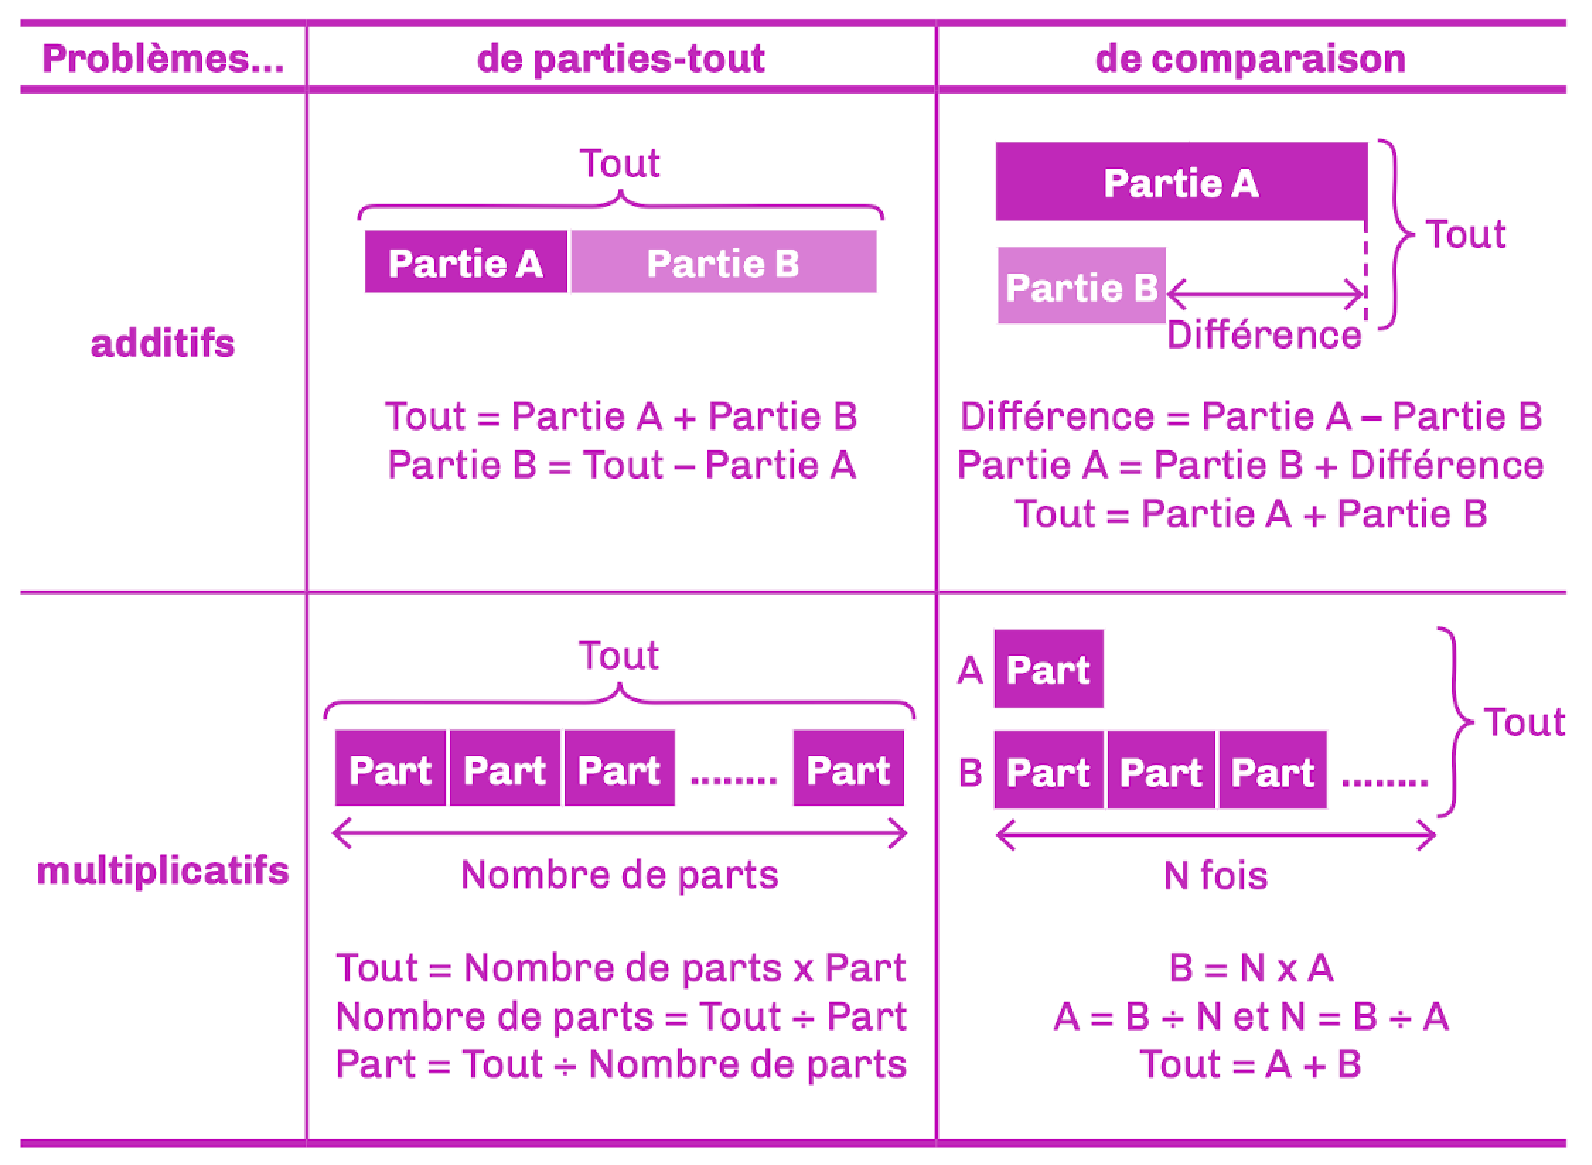
\includegraphics[width=11cm]{Nombres_et_calculs_did/Images/Num2_cours_barres}
\end{center}

La résolution de problèmes en {\bf plusieurs étapes} peuvent s’appuyer sur des schémas en barres à un ou plusieurs schémas selon le cas. \medskip

Quant aux problèmes algébriques, leur modélisation par des barres permettra ensuite, au cycle 4, de transiter petit à petit vers une modélisation algébrique.

\begin{exemple*1}
   {\small Dans un bocal, un enfant a des billes vertes, des billes rouges et des billes bleues. Il a 4 fois plus de billes rouges que de billes vertes et il a 3 billes vertes de plus que de billes bleues. En tout il a 51 billes. Combien a-t-il de billes de chaque couleur ?}
\end{exemple*1}

\begin{pspicture}(0,4)(17,7.5)
   \psframe(3,4.75)(2.5,5.25)
   \psarc(6.75,4.75){0.25}{-90}{0}
   \psline(7,4.75)(7,5.5)
   \psarc(7.25,5.5){0.25}{90}{180}
   \psarc(7.25,6){0.25}{180}{-90}
   \psline(7,6)(7,6.75)
   \psarc(6.75,6.75){0.25}{0}{90}
   \rput[l](0.5,5){Bleues}
   \rput[l](2.7,5){3}
   \rput[l](0.5,5.75){Rouges}
   \rput[l](0.5,6.5){Vertes}
   \rput[l](7.5,5.75){51 billes}
   \rput[l](9.5,7){On ajoute trois billes bleues pour compléter}
   \rput[l](9.5,6.5){la barre \og bleues \fg{} : $51+3 =54$.}
   \rput[l](9.5,5.75){On en déduit la valeur d'une barre : $54\div6 =9$.}
   \rput[l](9.5,5){Il y a 9 billes vertes, $4\times9$ billes = 36 billes rouges}
   \rput[l](9.5,4.5){et 9 billes $-$ 3 billes = 6 billes bleues.}
   \psset{fillstyle=solid,fillcolor=lightgray}         
      \psframe(2,4.75)(2.5,5.25)   
      \psframe(2,5.5)(3,6)
      \psframe(3,5.5)(4,6)
      \psframe(4,5.5)(5,6)
      \psframe(5,5.5)(6,6)      
      \psframe(2,6.25)(3,6.75)   
\end{pspicture}
         
\newpage


%%%%%%%%%%%%%%%%%%%%%%%%%%%%%%%%%%
\subsection{Analyse des difficultés des élèves, pistes de remédiation} 

\medskip

{\hautab{1.45}
\begin{Ltableau}{\linewidth}{2}{p{8cm}|p{7.96cm}}
   \hline
   \multicolumn{2}{|c|}{\cellcolor{FondTableaux}Pregnance de certaines règles du contrat didactique} \\
   \hline
   \og Dans un bateau il y a 25 chèvres et 12 moutons. Quel est l'âge du capitaine ? \fg{} Certains élèves répondent 37 ans dictés par les règles du contrat didactique : un problème de mathématiques a toujours une solution, et on attend de moi que je pose des opérations. L'élève ne cherche pas à donner du sens au problème, il se centralise sur les indices numériques.
   &
   {\it Il s'agit dans ce cas de \og casser \fg{} ces règles en proposant de temps à autre aux élèves des problèmes sans solution, des problèmes avec des données supplémentaires, des problèmes qui n'utilisent pas les dernières opérations étudiées\dots \newline
   On peut également proposer une solution d'un problème dont il faut qu'ils reconstituent l'énoncé.} \\
   \hline
   \multicolumn{2}{|c|}{\cellcolor{FondTableaux}La prégnance de mots inducteurs} \\
   \hline
   Certains mots comme \og chaque, range, total, reste, plus \fg\dots{} amènent les élèves à mobiliser certaines opérations quelles que soient les autres informations de l'énoncé.
   &
   {\it Il s'agit ici de faire prendre conscience à l'élève que les mots inducteurs peuvent conduire à des résultats faux. Pour cela on peut leur proposer par exemple un problème contenant le mot \og plus \fg{} et qui se résout à l'aide d'une soustraction.} \\
   \hline     
   \multicolumn{2}{|c|}{\cellcolor{FondTableaux}La surcharge de la mémoire de travail} \\
   \hline
   -- Difficultés à déchiffrer les mots. Arrivé au bout de sa lecture il aura perdu la plupart des informations de l'énoncé. \newline
   -- Essai de tout mémoriser. Lorsque sa mémoire de travail sera saturée, des indices seront oubliés.
   &
   {\it -- Une remédiation se situe au niveau de l'automatisation de la lecture, on peut proposer des énoncés présentés sous forme de situations concrètes ou faire lire le problème à haute voix. \newline
   -- On peut à l'élève de schématiser ou de \og raconter le problème \fg.} \\
   \hline
   \multicolumn{2}{|c|}{\cellcolor{FondTableaux}Le contexte du problème ou la présence de mots inconnus} \\
   \hline
   Un contexte trop éloigné du contexte social de l'élève ou un énoncé contenant des mots inconnus ne permet pas de juger de la compétence à résoudre un problème.
   &
   {\it L'enseignant doit choisir les mots de façon à ce que le contexte soit suffisamment familier pour les élèves et s'assurer que les mots en présence dans le texte sont connus.} \\
   \hline
   \multicolumn{2}{|c|}{\cellcolor{FondTableaux}Les blocages psychologiques} \\
   \hline
   Certains élèves se considèrent nuls en maths et pensent qu'ils sont incapables de résoudre un problème.
   &
   {\it Il s'agit de redonner confiance à l'élève, de lui faire prendre conscience qu'il est capable de faire quelque chose en maths.} \\
   \hline
   \multicolumn{2}{|c|}{\cellcolor{FondTableaux}L'insuffisance des réseaux de connaissance stockés dans la mémoire à long terme} \\
   \hline
   Le stockage des expériences n'est pas identique pour tous, ni la manière de les réactiver au moment opportun. De plus les expériences sociales ne sont pas les mêmes pour tous les élèves.
   &
   {\it L'enseignant doit être capable de sélectionner un certain nombre de problèmes permettant d'aider les élèves à les mémoriser correctement pour qu'ils deviennent des problèmes de référence.} \\
   \hline
   \multicolumn{2}{|c|}{\cellcolor{FondTableaux}La non maîtrise d'une technique opératoire} \\
   \hline
   Certains élèves élaborent une procédure de recherche correcte mais font des erreurs au moment d'effectuer le calcul.
   &
   {\it Faire un travail sur l'acquisition des algorithmes opératoires. Parallèlement, autoriser les élèves à utiliser leur calculatrice.} \\
   \hline
\end{Ltableau}}

\vfill\hfill{\it\footnotesize Source : travaux de R. Charnay et M. Mante, Les étapes de la résolution d'un problème, Mathématiques Tome 1, Hatier concours [char13-1].}


%%%%%%%%%%%%%%%%%%%%%%%%%%%%%
%%%%%%%%%%%%%%%%%%%%%%%%%%%%%
\activites

\textcolor{G1}{Sujet n°5 de l'épreuve de leçon, concours CRPE 2022, académie de Montpellier.} \\

{\bf\uline{Consigne candidat}} : À partir du sujet et du dossier proposés par le jury, vous concevrez la mise en œuvre d'une séance d'enseignement à l'école primaire dans chacune des deux disciplines français et mathématiques. Vous présenterez successivement les composantes pédagogiques et didactiques de chaque séance et son déroulement. \\

{\bf\uline{Sujet}} : Manipulation, représentation et verbalisation pour un passage progressif à l'abstraction. \\

{\bf\uline{Contexte de la séance d'enseignement}} : \\
   \hspace*{5mm} -- cycle d'enseignement : cycle 2 ; \\
   \hspace*{5mm} -- niveau de la classe : CP ; \\
   \hspace*{5mm} -- positionnement de la séance de mathématiques : \\
      \hspace*{10mm} -- période : période 2 ; \\
      \hspace*{10mm} -- séquence dans laquelle elle s'insère : résolution de problèmes. \\ [10mm]

{\bf\uline{Documents fournis au candidat}} : \\

{\bf\uline{Document 1}} : Ministère de I'Éducation nationale, de la Jeunesse et des Sports, extrait du BO n°11 du 26.11.2015, Annexe 1 : Programme d'enseignement du cycle des apprentissages fondamentaux (cycle 2) -- Volet 3 : les enseignements -- Mathématiques -- pp. 55-56.

\begin{center}
   \begin{minipage}{15cm}
      \textsf{[...] Au cycle 2, la résolution de problèmes est au centre de l'activité mathématique des élèves, développant leurs capacités à chercher, raisonner et communiquer. [...] Ils peuvent être issus de situations de vie de classe ou de situations rencontrées dans d'autres enseignements [...] ce qui contribue à renforcer le lien entre les mathématiques et les autres disciplines. [...] La composante écrite de l'activité mathématique devient essentielle. Ces écrits sont d'abord des écritures et représentations produites en situation par les élèves eux-mêmes qui évoluent progressivement avec l'aide du professeur vers des formes conventionnelles institutionnalisées dans les cahiers par des traces écrites qui ont valeur de référence.[...] L'introduction et l'utilisation des symboles mathématiques sont réalisés au fur et à mesure qu'ils prennent sens dans des situations basées sur des manipulations, en relation avec le vocabulaire utilisé, assurant une entrée progressive dans I'abstraction.[...]}
  \end{minipage}
\end{center}

\newpage

{\bf\uline{Document 2}} : Ministère de I'Éducation nationale, de la Jeunesse et des Sports, Guide fondé sur l'état de la recherche \og {\it Pour enseigner les nombres, le calcul et la résolution de problèmes au CP} \fg, juillet 2021, p. 84.

\begin{center}
   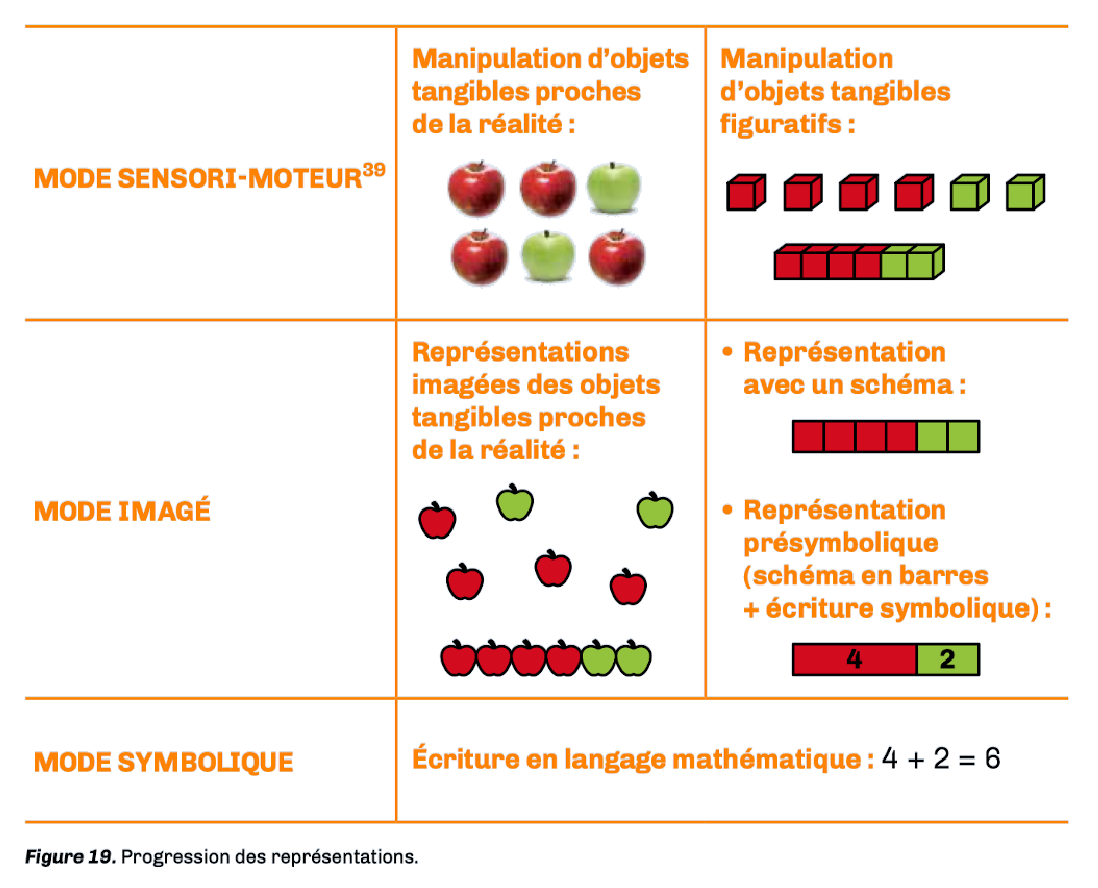
\includegraphics[width=11.5cm]{Nombres_et_calculs_did/Images/Num2_crpe_pommes_cubes}
\end{center}

\medskip

{\bf\uline{Document 3}} : Production d'un élève de CP, période 2, séance 3. \\

\fbox{\begin{minipage}{6cm}
   \flushleft Voici la production d'un élève réalisée lors de la troisième séance d'une séquence de cinq séances. \\
   La première séance était une mise en situation en extérieur, durant laquelle 7 élèves ont constaté qu'il manquait 2 vélos pour que chacun puisse en faire simultanément. La deuxième séance était une séance de manipulation d'images.
\end{minipage}}
\qquad
\begin{minipage}{11cm}
   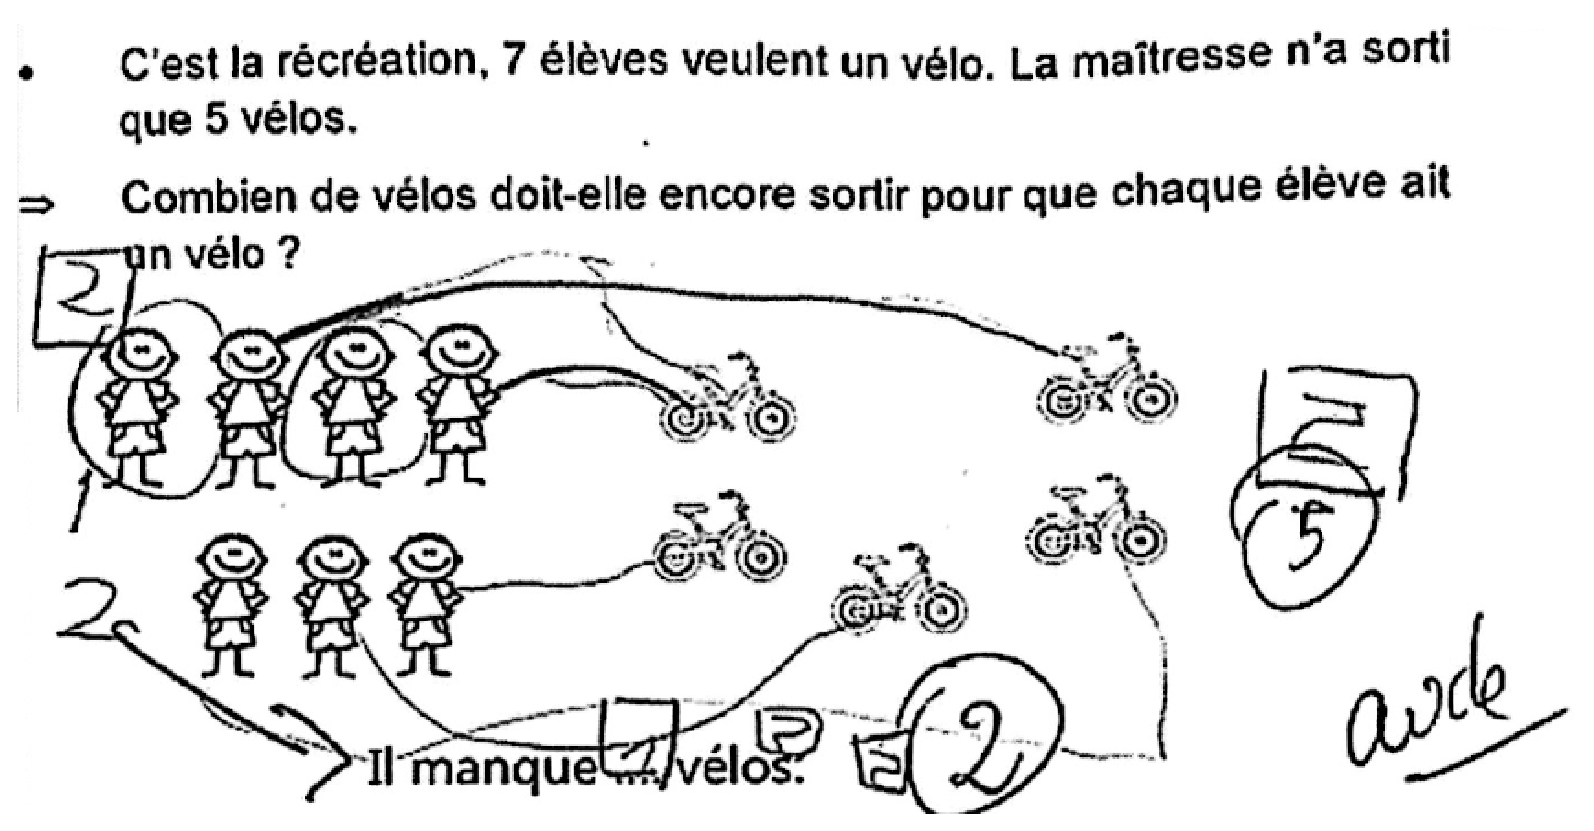
\includegraphics[width=10.5cm]{Nombres_et_calculs_did/Images/Num2_crpe_velos}
\end{minipage}

\ \\

{\bf\uline{Document 4}} : Production d'un élève de CP, période 2, séance 5. \\

\fbox{\begin{minipage}{6cm}
   Après une séance 4 d'introduction d'une représentation avec schéma, la séance 5 a conduit à ce type de production :
\end{minipage}}
\qquad
\begin{minipage}{8cm}
   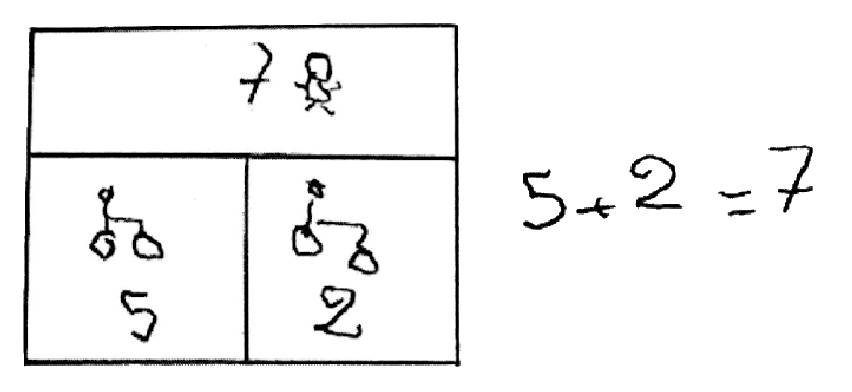
\includegraphics[width=7.5cm]{Nombres_et_calculs_did/Images/Num2_crpe_velos_bis}
\end{minipage}



%%%%%%%%%%%%%%%%%%%%%%%%%%%
%%%%%%%%%%%%%%%%%%%%%%%%%%%
\analyses

\begin{exercice}[Étude d'exercices de calcul mental]
{\it Ces exemples sont issus du livre de François BOULE \og Le calcul mental au quotidien \fg, aux éditions Canopé}

\begin{center}
\fbox{
\begin{minipage}{16cm}
\begin{itemize}
   \item {\bf Exercice 1.} \\
   Barrer les paires de nombres dont le quotient est 3. Quel est le nombre qui reste ?
   \medskip
   \begin{center}
   {\psset{unit=1.25}
   \begin{pspicture}(0,0.2)(1.8,1.8)
      \multido{\n=0+.6}{4}{\psline(\n,0)(\n,1.8)}
      \multido{\n=0+.6}{4}{\psline(0,\n)(1.8,\n)}
      \rput(.3,1.5){$8$ } \rput(.9,1.5){$39$ } \rput(1.5,1.5){$72$ } 
      \rput(.3,.9){$27$ } \rput(.9,.9){$23$ } \rput(1.5,.9){$69$ } 
      \rput(.3,.3){$13$ } \rput(.9,.3){$81$ } \rput(1.5,.3){$24$ } 
   \end{pspicture}
   \quad
   \begin{pspicture}(0,0.2)(1.8,1.8)
      \multido{\n=0+.6}{4}{\psline(\n,0)(\n,1.8)}
      \multido{\n=0+.6}{4}{\psline(0,\n)(1.8,\n)}
      \rput(.3,1.5){$14$ } \rput(.9,1.5){$17$ } \rput(1.5,1.5){$39$ } 
      \rput(.3,.9){$57$ } \rput(.9,.9){$48$ } \rput(1.5,.9){$51$ } 
      \rput(.3,.3){$16$ } \rput(.9,.3){$13$ } \rput(1.5,.3){$42$ } 
   \end{pspicture}
   \quad
   \begin{pspicture}(0,0.2)(1.8,1.8)
      \multido{\n=0+.6}{4}{\psline(\n,0)(\n,1.8)}
      \multido{\n=0+.6}{4}{\psline(0,\n)(1.8,\n)}
      \rput(.3,1.5){$11$ } \rput(.9,1.5){$54$ } \rput(1.5,1.5){$48$ } 
      \rput(.3,.9){$16$ } \rput(.9,.9){$24$ } \rput(1.5,.9){$51$ } 
      \rput(.3,.3){$33$ } \rput(.9,.3){$17$ } \rput(1.5,.3){$18$ } 
   \end{pspicture}}
   \end{center}
   \medskip
   \item {\bf Exercice 2.} \\
   Combiner les quatre nombres \og 1, 5, 7, 25\fg{} avec des signes arithmétiques \og $+,-,\times,\div$ \fg{} pour obtenir le nombre indiqué : \hspace*{3cm} \pscirclebox{10} ; \pscirclebox{11} ; \pscirclebox{60} ; \pscirclebox{13}.
   \item {\bf Exercice 3.} \\
   Combiner quatre fois le nombre \og 9 \fg{} avec des signes arithmétiques, pour obtenir le nombre indiqué.
   \begin{center}
   \pscirclebox{\;8\;} ; \pscirclebox{10} ; \pscirclebox{11} ; \pscirclebox{17} ; \pscirclebox{19} ; \pscirclebox{72} ; \pscirclebox{90} ; \pscirclebox{720}. 
   \end{center}
   \medskip
   \item {\bf Exercice 4.} \\
   Entourer le résultat exact, sans poser l'opération.
   \medskip
   \begin{center}
   {\renewcommand{\arraystretch}{1.3}
   \begin{tabular}{|c|c|c|c|c|}
      \hline
      17 $\times$ 8 & 631 & 136 & 361 & 163 \\
      \hline
      25 $\times$ 2,7 & 675 & 5,76 & 67,5 & 6,75 \\
      \hline
      51 $\times$ 0,15 & 7,65 & 5,76 & 76,5 & 0,65 \\
      \hline
      4,7 $\times$ 0,4 & 18,8 & 8,81 & 1,88 & 8,11 \\
      \hline
      0,03 $\times$ 2,2 & 0,66 & 0,066 & 6,06 & 0,606 \\
      \hline
   \end{tabular}}
   \end{center}
   \medskip
   \item {\bf Exercice 5.} \\
   Entourer le nombre le plus proche du résultat, sans le calculer.
   \medskip
   \begin{center}
   {\renewcommand{\arraystretch}{1.3}
   \begin{tabular}{|c|c|c|c|c|}
      \hline
      41 $\times$ 153 & 6200 & 600 & 200 & 5000 \\
      \hline
      0,2 $\times$ 8 & 8 & 0,8 & 4 & 1,5 \\
      \hline
      0,3 $\times$ 0,3 & 0,3 & 0,1 & 0,9 & 0,33 \\
      \hline
      0,7 $\times$ 124 & 70 & 8 & 100 & 800 \\
      \hline
      48 $\times$ 0,48 & 230 & 4,8 & 48 & 20 \\
      \hline
      54 $\div$ 0,1 & 0,5 & 5 & 50 & 500 \\
      \hline
   \end{tabular}}
   \smallskip
   \end{center}
\end{itemize}
\end{minipage}}
\end{center}
\begin{enumerate}
   \item Résoudre ces problèmes.
   \item Identifier la procédure utilisée à chaque fois.
   \item En quoi ces activités, qui utilisent un support écrit, relèvent-elles bien du calcul mental ?
   \item À quel niveau peuvent-elles être proposées ?
   \item Identifier, pour chacune d'elles, la ou les connaissances/compétences  travaillées.
   \item Dans la dernière activité, quel problème peut poser le calcul de $0,7\times 124$ ?
Comment le traiter avec les élèves ?
\end{enumerate}
\medskip
\end{exercice}

\begin{corrige}
\ \\ [-5mm]
\begin{enumerate}
   \item Réponses aux petits problèmes :
   \begin{itemize}
      \item Exercice 1 : il reste {\bf 8} ou {\bf 72} dans le premier tableau, {\bf 57} dans le second et {\bf 24} dans le dernier.
      \item Exercice 2 : $1 \times 7 \times 5 - 25 =$ {\bf 10}. \\
        \hspace*{1.9cm} $25 \div 5 - 1 + 7 =$ {\bf 11}. \\
        \hspace*{1.9cm} $7 \times 5 \times 1 + 25 =$ {\bf 60} \quad ou \quad $(7 \times 5) + (25 \times 1) =$ {\bf 60}. \\
        \hspace*{1.9cm} $(25-5-7) \times 1 =$ {\bf 13} ou $25 \div 5 + 7 +1 =$ {\bf 13} ou $(25 + 1) \div (7 - 5) =$ {\bf 13} ou $(25 - 7) \times 1 - 5 =$ {\bf 13}.
      \item Exercice 3 :
      \vspace*{-0.5cm}
      \begin{multicols}{3}
         $(9\times9-9)\div9=$ \bf{8}. \\
         $(9\times9+9)\div9=$ \bf{10}. \\
         $(9+9)\div9+9=$ \bf{11}. \\
         $9+9-(9\div9)=$ \bf{17}. \\
         $9+9+(9\div9)=$ \bf{19}. \\
         $(9-(9\div9))\times9=$ \bf{72}. \\
         $(9+(9\div9))\times9=$ \bf{90}. \\
         $9\times9\times9-9=$ \bf{720}.
      \end{multicols}
      \vspace*{-0.3cm}
      \item Exercice 4 : on trouve respectivement : {\bf 136 \; ; \; 67,5 \; ; \; 7,65 \; ; \; 1,88 \; et \; 0,066}.
      \item Exercice 5 : on trouve respectivement : {\bf 6\,200 \; ; \; 1,5 \; ; \; 0,1 \; ; \; 100 \; ; \; 20 \; et \; 500}.
   \end{itemize}
   \item Procédures possibles.
   \begin{itemize}
      \item Exercice 1 : résoudre des multiplications à trous par 3 : on utilise les plus petits nombres que l'on multiplie par 3 pour voir si la réponse est dans le carré ou division des plus grands nombres par 3, mais la procédure est plus difficile.
      \item Exercices 2 et 3 : procéder par essais-erreurs pour trouver l'un des résultats, à faire éventuellement en groupes pour plus de facilité.
      \item Exercice 4 : commencer par calculer le dernier chiffre du nombre pour trouver la réponse, ou éliminer des solutions, puis faire un calcul approximatif pour trancher entre plusieurs possibilités.
      \item Exercice 5 : effectuer un calcul en approchant chacun des deux nombres. Pour certains nombres décimaux, commencer par effectuer le calcul avec des valeurs entières puis appliquer les règles de division ou de multiplication par 10 ou 100. 
   \end{itemize}   
   \item Pour pouvoir résoudre ces problèmes dans un temps raisonnable, il faut faire l'essentiel des calculs mentalement. L'écrit sert à communiquer l'énoncé, à donner la réponse, mais parfois aussi, comme dans le problème 2 à trouver les différentes étapes d'un calcul en soulageant la mémoire.
   \item Niveau.
   \begin{itemize}
      \item Exercice 1 : à partir du cycle 2.
      \item Exercices 2 et 3 : à partir du cycle 3, à cause des parenthèses et de la complexité des calculs.
      \item Exercices 4 et 5 : à partir du cycle 3, à cause des nombres décimaux et des calculs approchés.
   \end{itemize}
   \item Connaissances et compétences travaillées.
   \begin{itemize}
      \item Exercice 1 : connaître les tables de multiplication de 2 à 9 ; savoir effectuer une multiplication à deux chiffres.
      \item Exercices 2 et 3 : connaître les tables d'addition et de multiplication de 2 à 9 ; effectuer un calcul mental en utilisant les signes arithmétiques.
      \item Exercices 4 et 5 : estimer l'ordre de grandeur d'un résultat, effectuer un calcul approché ou exact.
   \end{itemize}
   \item Deux réponses sont tout à fait légitimes dans cette activité sur le calcul approché : 70 et 100. En effet $0,7 \times 124$ est proche de $0,7 \times 100$, mais $0,7 \times 124$ est plus grand que 70, donc 100 paraît aussi un bon candidat. Le calcul exact donne 86,8 qui est presque la moyenne exacte de 70 et de 100,  les deux réponses peuvent être considérées comme exactes car l'objectif de cette activité est de faire faire un calcul approché aux élèves.
   \end{enumerate}
\end{corrige}

\clearpage


\begin{exercice}[CRPE 2018 G2]
Lors d’un travail sur le calcul en ligne, un enseignant propose la situation suivante à ses élèves : \og Calculer $5\times68$ \fg. \\
Voici les productions de quatre élèves, Robin, Eléonore, Lucie et Mathys. \\ [2mm]
   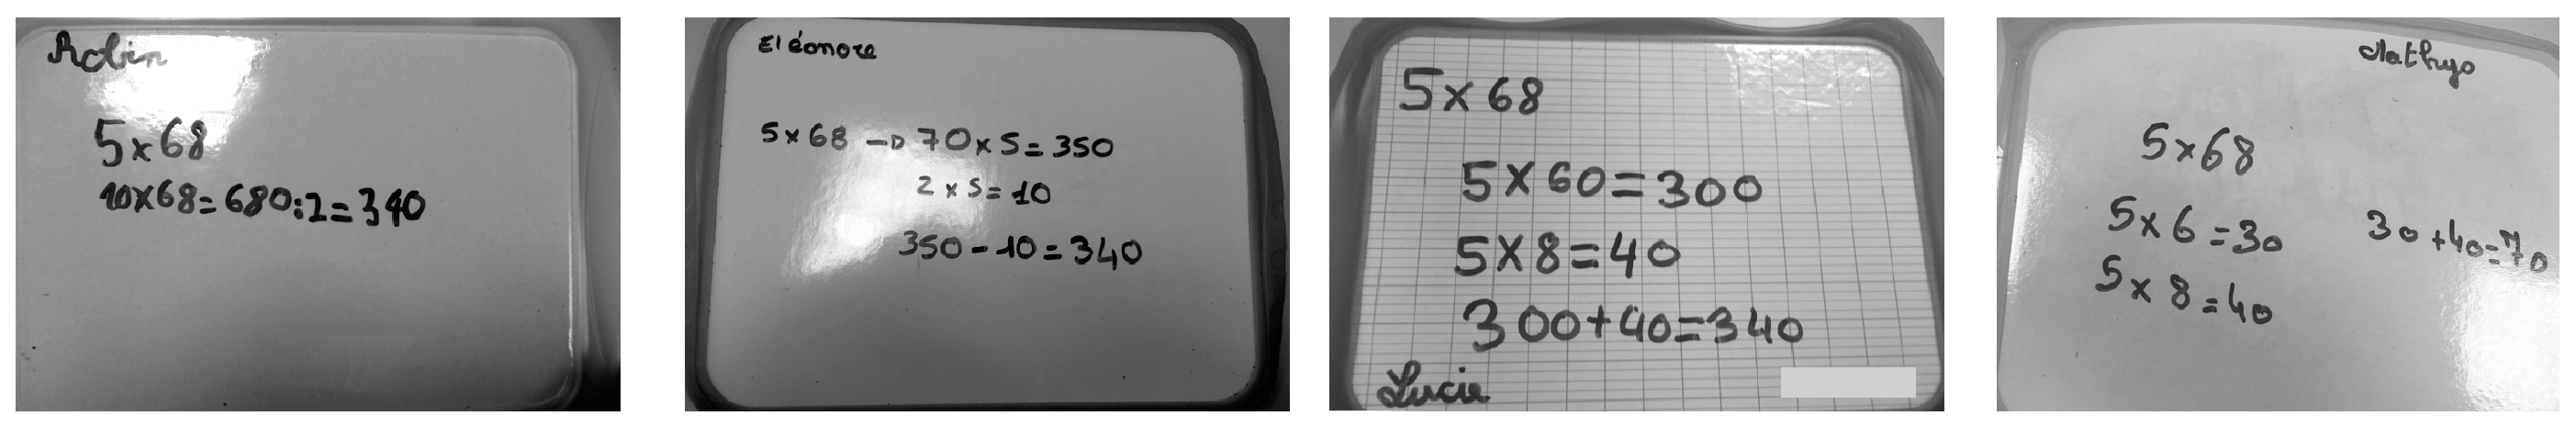
\includegraphics[width=17cm]{Nombres_et_calculs_did/Images/Num2_analyse_5x8}
\begin{enumerate}
   \item Analyser chacune des productions, en explicitant les procédures mises en oeuvre et en relevant les éventuelles erreurs.
   \item Donner trois démarches pouvant être attendues d’un élève de cycle 3 pour calculer en ligne $25\times28$. \\
   Pour chacune de ces démarches indiquer les connaissances en jeu.
\end{enumerate}
\end{exercice}

\begin{corrige}
\ \\ [-5mm]
\begin{enumerate}
   \item Analyse des productions d'élèves :
   \begin{itemize}
      \item {\bf Robin.} Il sait que multiplier par 5 revient à multiplier par 10, puis à diviser par 2. \\
      Il commence par calculer $10\times68$ car il sait effectuer une multiplication par 10 mentalement, il obtient 680. Puis il divise par 2 et trouve 340. \\
      Son résultat et sa procédure sont justes, il y a cependant une erreur d'écriture puisqu'il écrit en ligne ses calculs à la suite, le statut du signe \og = \fg{} n'est alors pas respecté puisqu'on peut lire \og $10\times68 =340$ \fg. Il aurait dû écrie $10\times68 =680$, puis $680\div2 =340$.
      \item {\bf Eléonore.} Elle passe par la décomposition de 68 comme $70-2$ puis elle utilise la distributivité de la multiplication par rapport à la soustraction. \\
      Elle effectue $70\times5 =350$ certainement en calculant mentalement que $7\times5 =35$ puis en \og ajoutant un zéro \fg{} afin d'effectuer la multiplication par 10. Ensuite, elle effectue le calcul $2\times 5 =10$ et enfin, elle soustrait ses deux résultats pour obtenir 340. \\
      Sa procédure et son résultat sont justes.
      \item {\bf Lucie.} Elle utilise la décomposition additive de 68 qui est $60+8$ puis elle utilise la distributivité de la multiplication sur l'addition. \\
      Elle effectue $5\times60 =300$ certainement en calculant mentalement que $5\times6 =30$ puis en \og ajoutant un zéro \fg{} afin d'effectuer la multiplication par 10. Ensuite, elle effectue le calcul $5\times8 =40$ et enfin, elle additionne ses deux résultats pour obtenir 340. \\
      Sa procédure et son résultat sont justes.
      \item {\bf Mathys.} Il utilise l'écriture de 68 en multipliant successivement 5 par 6 ce qui donne 30 et 5 par 8 ce qui donne 40 puis il additionne ces deux résultats. \\
      Sa procédure aurait pu être correcte s'il avait pensé que $5\times6$ correspondait au nombre de dizaines mais il ne semble pas avoir conscience de la signification de l'écriture positionnelle de notre système de numération puisqu'il considère le 6 des dizaines et le 8 des unités de la même manière. Son résultat est faux.
   \end{itemize}
   \item Voici quelques démarches possibles par un élève de cycle 3 : \\ [3mm]
\begin{tabular}{|p{4.8cm}|p{5.2cm}|p{4.6cm}|}
      \hline
      Calculs. & Démarche. & Connaissances. \\
      \hline
      $100\times28 =2\,800$ \newline
      $2\,800\div2 =1\,400$ \newline
      $1\,400\div2 =700$.
      &
      25 c'est 100 divisé par 4 ; diviser par 4, c'est diviser par 2 puis encore diviser par 2. 
      &
      Multiplication par 100, division par 2 (prendre la moitié). \\
      \hline
      $100\times28 =2\,800$ \newline
      $2\,800\div4 =700$.
      &
      Multiplier par 25, c'est multiplier par 100 puis diviser par 4.
      &
      Multiplication par 100, \newline
      division par 4 (table des 4). \\
      \hline
      $28 =30-2$ \newline
      $25\times30 =750$ \newline
      $25\times2 =50$ \newline
      $750-50 =700$
      &
      Décomposition de 28 à partir de la dizaine la plus proche 30,  multiplication par 25 de 30 et 2, soustraction des résultats.
      &
      Décomposition d'un nombre, multiplication par 25 de nombre simples, distribution de la multiplication sur la soustraction. \\
      \hline
      $25\times28 =(20+5)\times(20+8)$ \newline
      $20\times20 =400$ \newline
      $20\times8 =160$ \newline
      $5\times20 =100$ \newline
      $5\times8 =40$ \newline
      $400+160+100+40 =700$
      &
      Décomposition additive des deux facteurs, calculs de tous les termes issus des multiplications, addition des résultas obtenus.
      &
      Décomposition additive, distributivité de la multiplication sur l'addition, multiplications par 2, 5 et 10. \\
      \hline
   \end{tabular}
\end{enumerate}
\end{corrige}

\bigskip


\begin{exercice}[CRPE 2001 Aix]
Vous trouverez ci-dessous un problème du cahier de l'Évaluation Nationale CE2, édition septembre 2000. Cet exercice a été proposé dans les classes de CE2 entre le 11 et le 20 septembre 2000.
\begin{center}
   \it
   \begin{minipage}{13cm}
   {\bf Problème :} 108 coureurs prennent le départ d'une course. Il y a beaucoup d'abandons. 85 coureurs seulement terminent la course. {\bf Combien de coureurs ont abandonné ?}
      \begin{center}
         \fbox{
         \begin{minipage}{10cm}
            Utilise ce cadre pour faire tes recherches. \\ [0.5cm]
         \end{minipage}}
      \end{center}
   {\bf Réponse :} \dotfill
   \end{minipage}
\end{center}
\begin{enumerate}
   \item Quelles sont les compétences mathématiques évaluées dans cet exercice ?
   \item Le problème peut être mis en équation de 3 manières différentes : indiquez-les.
   \item Vous trouverez page suivante les productions de 11 enfants.
   \begin{enumerate}
      \item Classez ces productions selon les procédures utilisées.
      \item Analysez les erreurs commises par Houssan et Benyamine.
   \end{enumerate}
   \item Voici les consignes de codage données pour cet exercice :
   \begin{center}
   \smallskip
   \hrule
   \smallskip
   Réponse exacte : 23 coureurs (avec ou sans l'unité) \dotfill code 1 \\
   Écriture soustractive exacte ($108-85$), mais résultat faux ou absent  \dotfill code 4 \\
   Mise en \oe uvre de l'addition \dotfill code 8 \\
   Autres résultats \dotfill code 9 \\
   Absence de réponse \dotfill code 0 \\
   \smallskip
   \hrule
   \smallskip
   \end{center}
En utilisant ces consignes :
\begin{itemize}
   \item Pour quels enfants mettriez vous le code 1 ?
   \item Quel code mettriez vous pour Cédric ? pour Camille ?
   \item Quelles remarques faites-vous sur les codes proposés ?
\end{itemize}
\end{enumerate}
\end{exercice}

\pagebreak


\begin{center}
   {\it Productions de l'exercice 2 : CRPE 2001 Aix} \\ [3mm]
   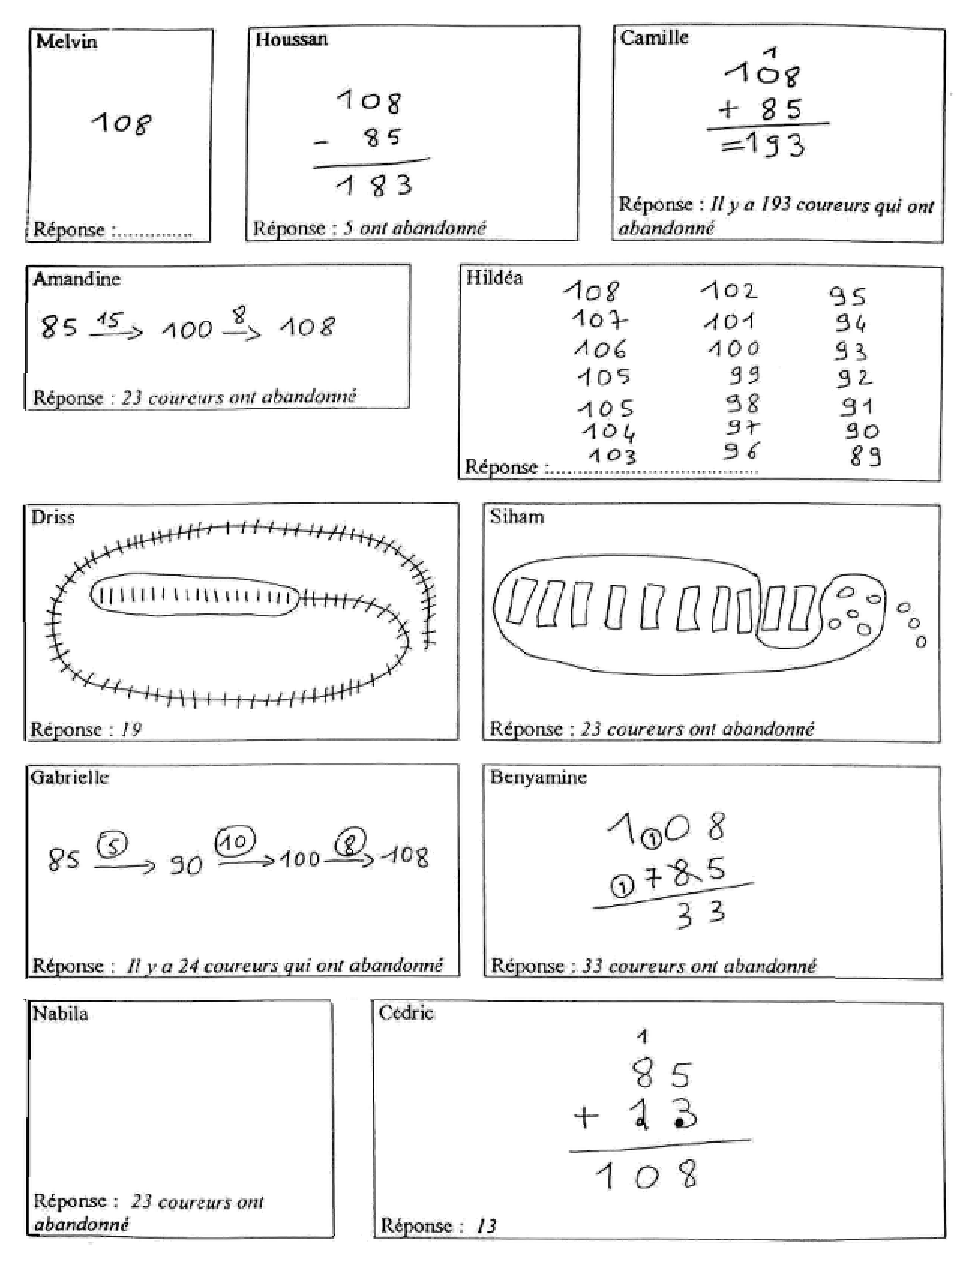
\includegraphics[width=16.5cm]{Nombres_et_calculs_did/Images/Num2_analyse_coureurs}
\end{center}

\begin{corrige}
\ \\ [-5mm]
\begin{enumerate}
   \item La principale compétence mathématique évaluée dans cet exercice est : \og Résoudre un problème relevant de la soustraction. \fg{}. Selon la typologie de {\it G. Vergnaud}, il s'agit d'un problème du champ additif de type \og transformation d'un état \fg, dans lequel l'état initial et l'état final sont connus ; on recherche la transformation. \\
   La compétence secondaire est : \og Effectuer une soustraction \fg{}. À la fin du CE1, les élèves doivent connaître et utiliser les techniques opératoires de l'addition et de la soustraction (sur des nombres inférieurs à 1\,000).
   \item Si $x$ désigne le nombre de coureurs ayant abandonné, on peut écrire : 
   \begin{itemize}
      \item $108-x = 85$ ;
      \item $85+x =108$ ;
      \item $108-85 = x$.
   \end{itemize}
   \item
   \begin{enumerate}
      \item On peut distinguer :
      \begin{itemize}
         \item les procédures {\bf non apparentes} de Melvin et de Nabila (le premier ne donne pas de réponse, la deuxième donne la réponse exacte sans aucune justification) ;
         \item les procédures traduisant une {\bf mauvaise compréhension de la situation} : Camille qui fait une modélisation erronée de la situation ;
         \item les procédures utilisant la {\bf schématisation} : celles de Driss et de Siham, dont la représentation est plus aboutie ;
         \item les procédure utilisant le {\bf décomptage} : celle d'Hilda ;
         \item les procédures de {\bf recherche du complément} : par sauts successifs pour Amandine et Gabrielle, par une addition à trous pour Cédric (qui fait une erreur de calcul) ;
         \item les procédures {\bf soustractives} d'Houssan et Benyamine qui se trompent dans leur calcul.
      \end{itemize}
   \item {\bf Erreur d'Houssan :} on peut envisager deux hypothèses principales :
  \begin{itemize}
   \item dans chaque colonne, il calcule l'écart entre le plus grand et le plus petit chiffre : $8-5= 3$ , $8-0= 8$ et $1-0= 1$ ;
   \item au lieu de soustraire, il additionne 108 et 85 et oublie la retenue.
   \end{itemize}   
   {\bf Erreur de Benyamine :} pas de problème apparent pour les unités. Pour la suite du calcul, il est difficile de recréer la chronologie. Ne pouvant ôter 8 de 0, il ôte 8 de 10 et place le 1 en bas (conservation des écarts). \\
   La présence du 7 indique très vraisemblablement qu'il a retranché 1 de 8 pour obtenir le 7. Mais ce 1 n'est pas le 1 entouré du bas, puisqu'il trouve 33 et non 133. Il semble donc que le 1 ajouté en haut soit traité doublement : pour la conservation des écarts d'abord, mais aussi par retrait au terme du bas.
   \end{enumerate}
   \setcounter{enumi}{3} 
   \item Les codes attendus.
   \begin{itemize}
      \item On mettra le code 1 à Amandine, Siham et Nabila qui ont donné la réponse attendue : 23.
      \item Cédric devrait recevoir le code 8 ou 9 selon si l'on considère que faire une addition à trou rentre dans la \og mise en \oe uvre de l'addition \fg.
      \item Camille devrait recevoir le code 8 si on se réfère à la procédure utilisée, mais au regard de sa réponse (193 coureurs), on pourrait penser au code 9.
      \item Les consignes de codage sont ambiguës : elles ne permettent pas de distinguer l'utilisation erronée de l'addition et l'utilisation pertinente de l'addition à trous. Le codage proposé ne permet pas de distinguer les erreurs relatives à la procédure de résolution du problème de celles relatives à la procédure de calcul. \\
   \end{itemize}
\end{enumerate}
\end{corrige}

\pagebreak


\begin{exercice}[CRPE 2018 G1]
\ \\ [-10mm]
\begin{enumerate}
   \item Donner deux raisons pour lesquelles le calcul en ligne est, en termes d’apprentissage, complémentaire au calcul posé.
   \item Le calcul suivant est proposé à des élèves de cycle 2 qui pratiquent régulièrement le calcul en ligne : $28+17=$ ? \\
   Expliciter trois stratégies qu’un élève de cycle 2 pourrait mobiliser pour effectuer ce calcul en ligne.
   \item Expliciter trois stratégies de calcul mental ou en ligne qu’un élève de cycle 2 pourrait mobiliser pour effectuer $14\times5$. Pour chacune, indiquer quelles sont les connaissances et les propriétés utilisées.
\end{enumerate}
\end{exercice}

\begin{corrige}
\ \\ [-5mm]
\begin{enumerate}
   \item Le calcul en ligne se pratique en amont du calcul posé (implicitement le calcul en colonnes), puis les deux pratiques sont menées en étroite relation. Elles sont complémentaires l'une de l'autre pour diverses raisons que l'on peut résumer dans un tableau : \\
   \medskip
   \begin{tabular}{|p{7cm}|p{7cm}|}
      \hline
      Calcul en ligne.
      &
      Calcul posé. \\
      \hline
      Procédure basée sur la {\bf réflexion}. \newline
      Les élèves travaillent les propriétés de notre numération ainsi que le sens des opérations et utilisent une procédure en fonction des nombres en jeu.
      &
      Procédure \og {\bf clé en main} \fg{}. \newline
      Mise en place d'un algorithme : succession d’étapes utilisées dans un certain ordre et de la même manière indépendamment des nombres en jeu. \\
      \hline
      Procédure de {\bf construction}. \newline
      Il développe des habiletés calculatoires des élèves ainsi que la construction et la connaissance de faits numériques et de propriétés élémentaires.
      &
      Procédure d'{\bf utilisation}. \newline
      Utilisation de ces faits numériques (par exemple les tables de multiplications) pour mener à bien des calculs posés. \\
      \hline
      Procédure {\bf rapide}. \newline
      Le calcul en ligne se travaille également en relation avec le calcul mental et permet d'effecteur des calculs assez rapidement tant qu'ils sont simples.
      &
      Procédure {\bf sûre}. \newline
      N'importe quelle opération classique peut être effectuée mais on ne peut pas agir sur le nombre d'étapes de l'algorithme afin de le réduire. \\
      \hline
   \end{tabular}
   \bigskip
   \item 
   \begin{itemize}
      \item Décomposition additive \og dizaine-unité \fg{} puis commutativité de l'addition : \\
      $28+17 =20+8+10+7 =20+10+8+7 =30+15 =45.$
      \smallskip
      \item Complément à la dizaine la plus proche puis commutativité : \\
      $28+17 =30-2+20-3 =30+20-2-3 =50-5 =45$.
      \smallskip
      \item Calcul de proche en proche en utilisant la décomposition additive : \\
      $28+17 = 28+10+7 =38+7 =45$ ou $28+17 = 28+2+15 =30+15 =45$. \\
   \end{itemize}
   \item En cycle 2, une partie du calcul mental s'effectue sur les nombres 1, 2, 5, 10\dots{}, on a donc par exemple les trois procédures suivantes : \\
   \medskip
   \begin{tabular}{|p{7cm}|p{7cm}|}
      \hline
      Connaissances. & Propriétés. \\
      \hline
      \multicolumn{2}{|c|}{$14\times5 =14\times10\div2 =140\div2 =70$} \\
      \hline
      Multiplication par 10. \newline Moitié (de 10 et de 140).
      &
      Associativité de la multiplication. \\
      \hline
      \multicolumn{2}{|c|}{$14\times5 =2\times7\times5 =2\times35 =70$} \\
      \hline
      Table du 5. \newline Double.
      &
      Associativité et commutativité de la multiplication. \\
      \hline
      \multicolumn{2}{|c|}{$14\times5 =10\times5+4\times5 =50+20 =70$} \\
      \hline
      Décomposition additive \og dizaine-unité \fg.\newline
      Table du 5.
      &
      Distributivité de la multiplication par rapport à l'addition. \\
      \hline
   \end{tabular}
\end{enumerate}
\end{corrige}

\bigskip


\begin{exercice}[CRPE 2018 G3]
Un professeur des écoles distribue le problème suivant à ses élèves de CE1 et leur demande de se mettre en groupe pour le résoudre. Les productions de quatre groupes sont présentées dans la suite.
\begin{center}
   \fbox{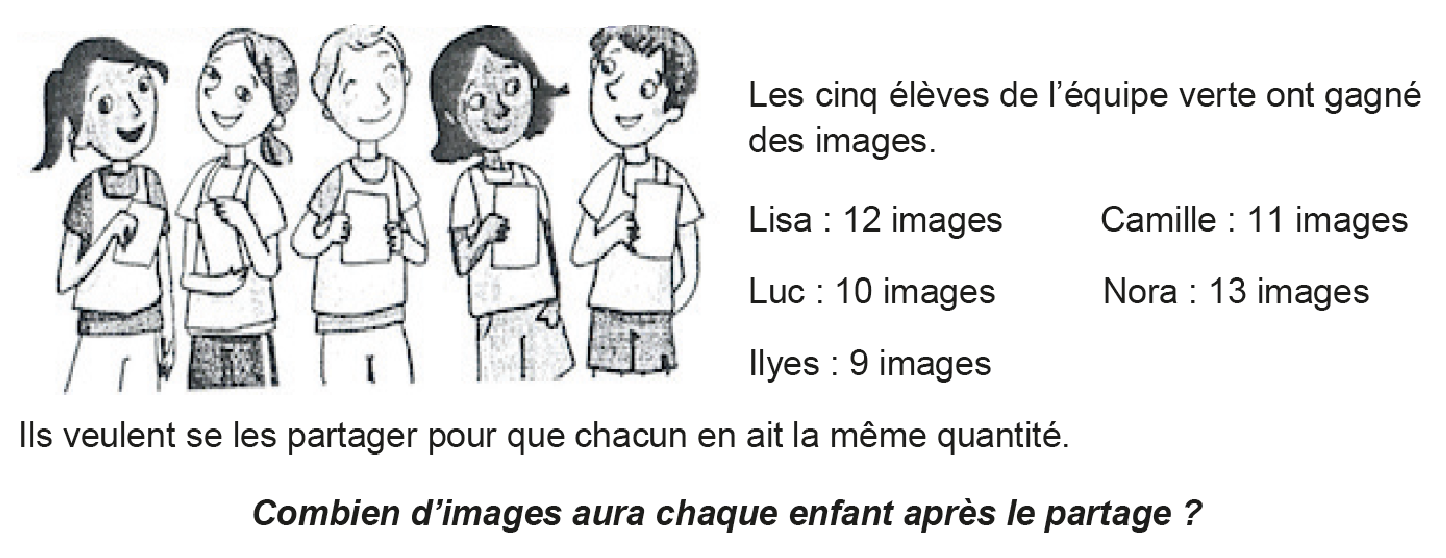
\includegraphics[width=13cm]{Nombres_et_calculs_did/Images/Num2_analyse_probleme_additif}}
\end{center}
\begin{enumerate}
   \item Citer deux objectifs d’apprentissage que cette situation permet de travailler.
   \item
   \begin{enumerate}
      \item Expliquer chacune des stratégies d’addition pour trouver 55 pour les élèves des groupes 1 et 2 en s’appuyant sur leurs productions ci-dessous.
      \item Donner un point commun et deux différences dans la démarche mathématique des groupes 1 et 2.
   \end{enumerate}
   \item Citer deux difficultés qu’a rencontrées le groupe 3.
\end{enumerate}
\end{exercice}

\fbox{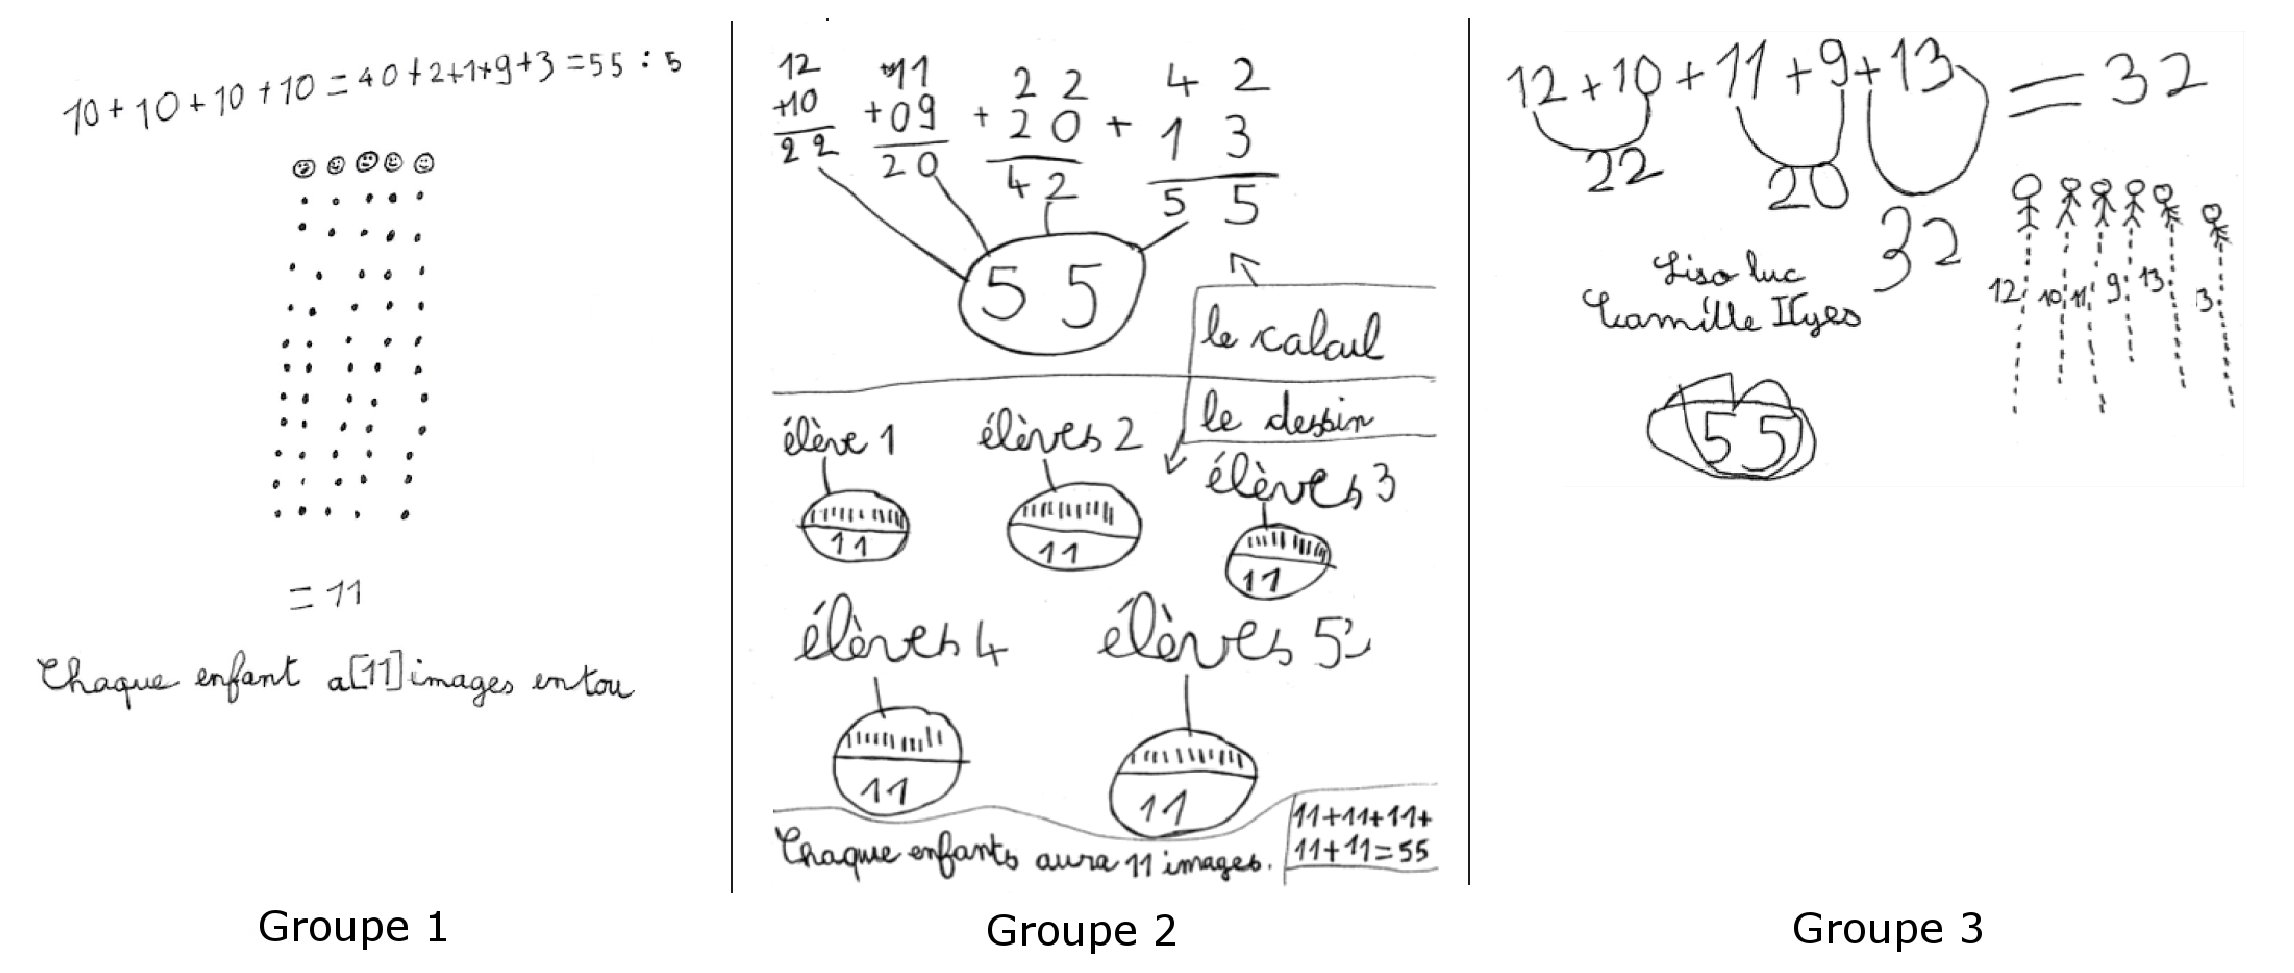
\includegraphics[width=17cm]{Nombres_et_calculs_did/Images/Num2_analyse_probleme_additif_groupes}}

\begin{corrige}
\ \\ [-5mm]
\begin{enumerate}
   \item On peut citer les objectifs d'apprentissage suivants :
   \begin{itemize}
      \item un objectif général : résolution d'un problème (en groupe) ;
      \item un objectif disciplinaire : travailler le champ additif (addition à cinq nombres) et une approche de la division partition.
   \end{itemize}
   \item Analyse des productions des groupes 1 et 2. \\
   \begin{enumerate}
      \item Au niveau des stratégies :
      \begin{itemize}
         \item pour le {\bf groupe 1}, les élèves ont additionné toutes les dizaines des nombres en présence, il y en a quatre ce qui fait 40, puis ils ont ajouté à ce nombre les unités restantes : 2 pour Lisa, 1 pour Camille, 9 pour Ilyes et 3 pour Nora. Ils ont trouvé 55 (cependant, l'écriture mathématique est incorrecte puisque les calculs sont faits les uns derrière les autres et le signe \og = \fg{} n'a pas son sens mathématique usuel) ;
         \item pour le {\bf groupe 2}, ils additionnent les nombres en présence par deux : tout d'abord Lisa et Luc, puis Camille et Ilyes. Ensuite, ils additionnent les deux résultats trouvés, et enfin ils additionnent le dernier nombre, celui de Nora.
      \end{itemize}
      \item Point commun et différences :
      \begin{itemize}
         \item {\bf point commun} : les deux groupes ont additionné les bonbons puis les ont puis \og partagés \fg{} grâce à un schéma ;
         \item {\bf différences} : au niveau de l'addition, le groupe 1 a séparé les dizaines et les unités alors que le groupe 2 a additionné les nombres un par un. \\
         Au niveau du partage, le groupe 1 a écrit la division $55:5$ et on a l'impression qu'il a trouvé la solution mentalement puis l'a vérifiée par un schéma (les lignes verticales formées par les points modélisant les bonbons semblent faites en une seule fois) alors que dans le groupe 2, il est possible qu'ils aient distribué un par un les bonbons aux cinq élèves jusqu'à 55 sans se poser la question de l'opération en jeu. La vérification se fait alors à la fin par un calcul en ligne.
      \end{itemize}
   \end{enumerate}
   \setcounter{enumi}{2} 
   \item Difficultés rencontrées par le groupe 3 :
   \begin{itemize}
      \item la première difficulté a été d'effectuer l'addition en ligne des cinq nombres : les élèves sont capables de faire des additions en ligne à deux chiffres (Lisa-Luc et Camille-Ilyes), mais ensuite ont du mal à trouver la somme totale qui est fausse. Ils ont fini par modéliser la situation par un schéma et compter un à un les bonbons ;
      \item la seconde difficulté provient de la résolution du problème : ils n'ont pas répondu à la question (parce qu'ils ne savaient pas le faire, ou parce qu'ils n'ont pas compris la consigne ?) et se sont arrêté au résultat 55 qu'ils ont encadré.
   \end{itemize}
\end{enumerate}
\end{corrige}


%%%%%%%%%%%%
\Recreation %%%%%%
%%%%%%%%%%%%

\setcounter{exercice}{0}


\begin{exercice*}[\fbox{C1} - Situation problème : les maisons] %%% 2
\begin{minipage}{8cm}
   Les enfants disposent de carrés et des triangles de papiers de même taille mais de 4 couleurs différentes. Ils doivent trouver toutes les maisons différentes qu’il est possible de fabriquer à partir de ce matériel.
\end{minipage}
\hspace*{1cm}
\begin{minipage}{6cm}
   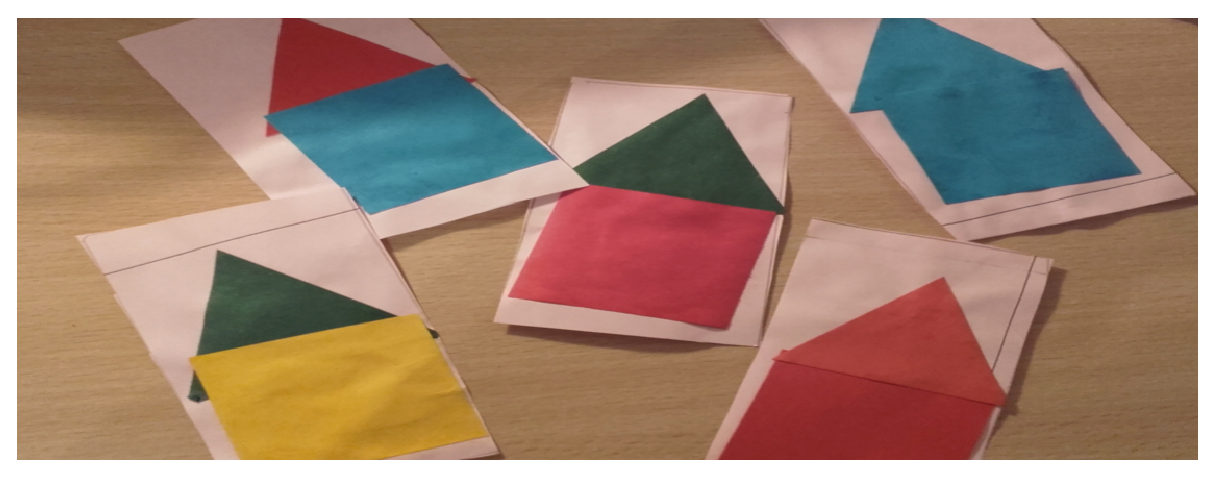
\includegraphics[width=6cm]{Nombres_et_calculs_did/Images/Num2_activites_maisons}
\end{minipage}

\bigskip

{\bf Objectif :} Apprendre à chercher, organiser sa recherche, trouver tous les possibles d’une situation.

\medskip

{\bf Compétences visées :}
\begin{itemize}
   \item Reproduire un assemblage à partir d’un modèle.
   \item Apprendre à chercher, organiser sa recherche, raisonner.
   \item Explorer les formes, les suites organisées.
   \item Catégoriser, classer.
\end{itemize}

\medskip

{\bf Matériel :}
\begin{itemize} 
    \item des carrés et des triangles de trois couleurs différentes ;
    \item une fiche pour la trace écrite finale avec des maisons vierges ;
    \item des feutres ou des crayons de couleur.
\end{itemize}

\medskip

{\bf Déroulement de l'activité :}
\begin{description}
  \item[Étape 1 :] {\bf Premiers essais de recherche individuelle.} \\
     Appropriation : présentation du matériel. Comment faire une petite maison avec ce matériel ? \\
     Recherche : vous allez essayer de construire le plus de maisons possibles, toutes différentes. \\
     Mise en commun : constater que certains camarades en ont plus ou moins que d’autres, que certains ont des maisons jumelles.
  \item[Étape 2 :] {\bf Organiser l'ensemble des possibles, trouver des caractères communs.} \\
     Appropriation : qu'a-t-on fait à l'étape 1 ? J'ai fabriqué toutes les possibilités, je vais vous les prêter et par équipes de 3, vous allez les organiser pour qu’on puisse vérifier quelles sont celles qui vous manquent. \\
     Recherche : verbalisation pour trouver un critère de regroupement. \\
     Mise en commun : dégager et expliquer le critère de tri.
  \item[Étape 3 :] {\bf Reprendre l'étape 1 en utilisant le critère d'organisation pour trouver les maisons qui manquent.} \\
     Appropriation : faire reformuler et expliciter. \\
     Réinvestissement : étayage pour soutenir par le langage la stratégie pour identifier les maisons manquantes. \\
     Trace finale : les 16 maisons sont affichées.
\end{description}

\medskip

\begin{center}
   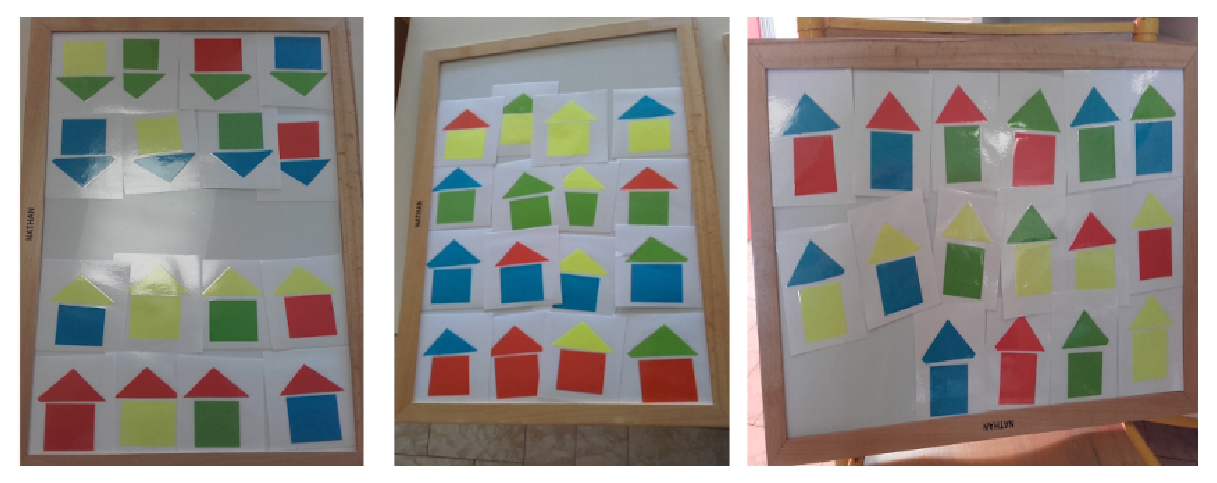
\includegraphics[width=14cm]{Nombres_et_calculs_did/Images/Num2_activites_maisons_organisation} 
\end{center}
\end{exercice*}


\begin{exercice*}[\fbox{C1} - Situation problème : L
les embouteillages] %%% 1
\begin{minipage}{8cm}
   Il s'agit d'une activité d'anticipation pour les MS et GS (peut être adapté pour la PS) proposée par {\it Dominique Valentin} dans son livre \href{http://www.editions-hatier.fr/livre/decouvrir-les-mathematiques-grande-section-ed-2015-guide-de-lenseignant}{\it\blue Découvrir le monde avec les mathématiques}. Ce jeu est une adaptation du jeu de société \og Ruch hour \fg{} qui dispose d'un quadrillage de 6 cases par 6 cases alors que le jeu adapté ne possède que 5 cases par 5 cases.
\end{minipage}
\hspace*{1cm}
\begin{minipage}{6cm}
   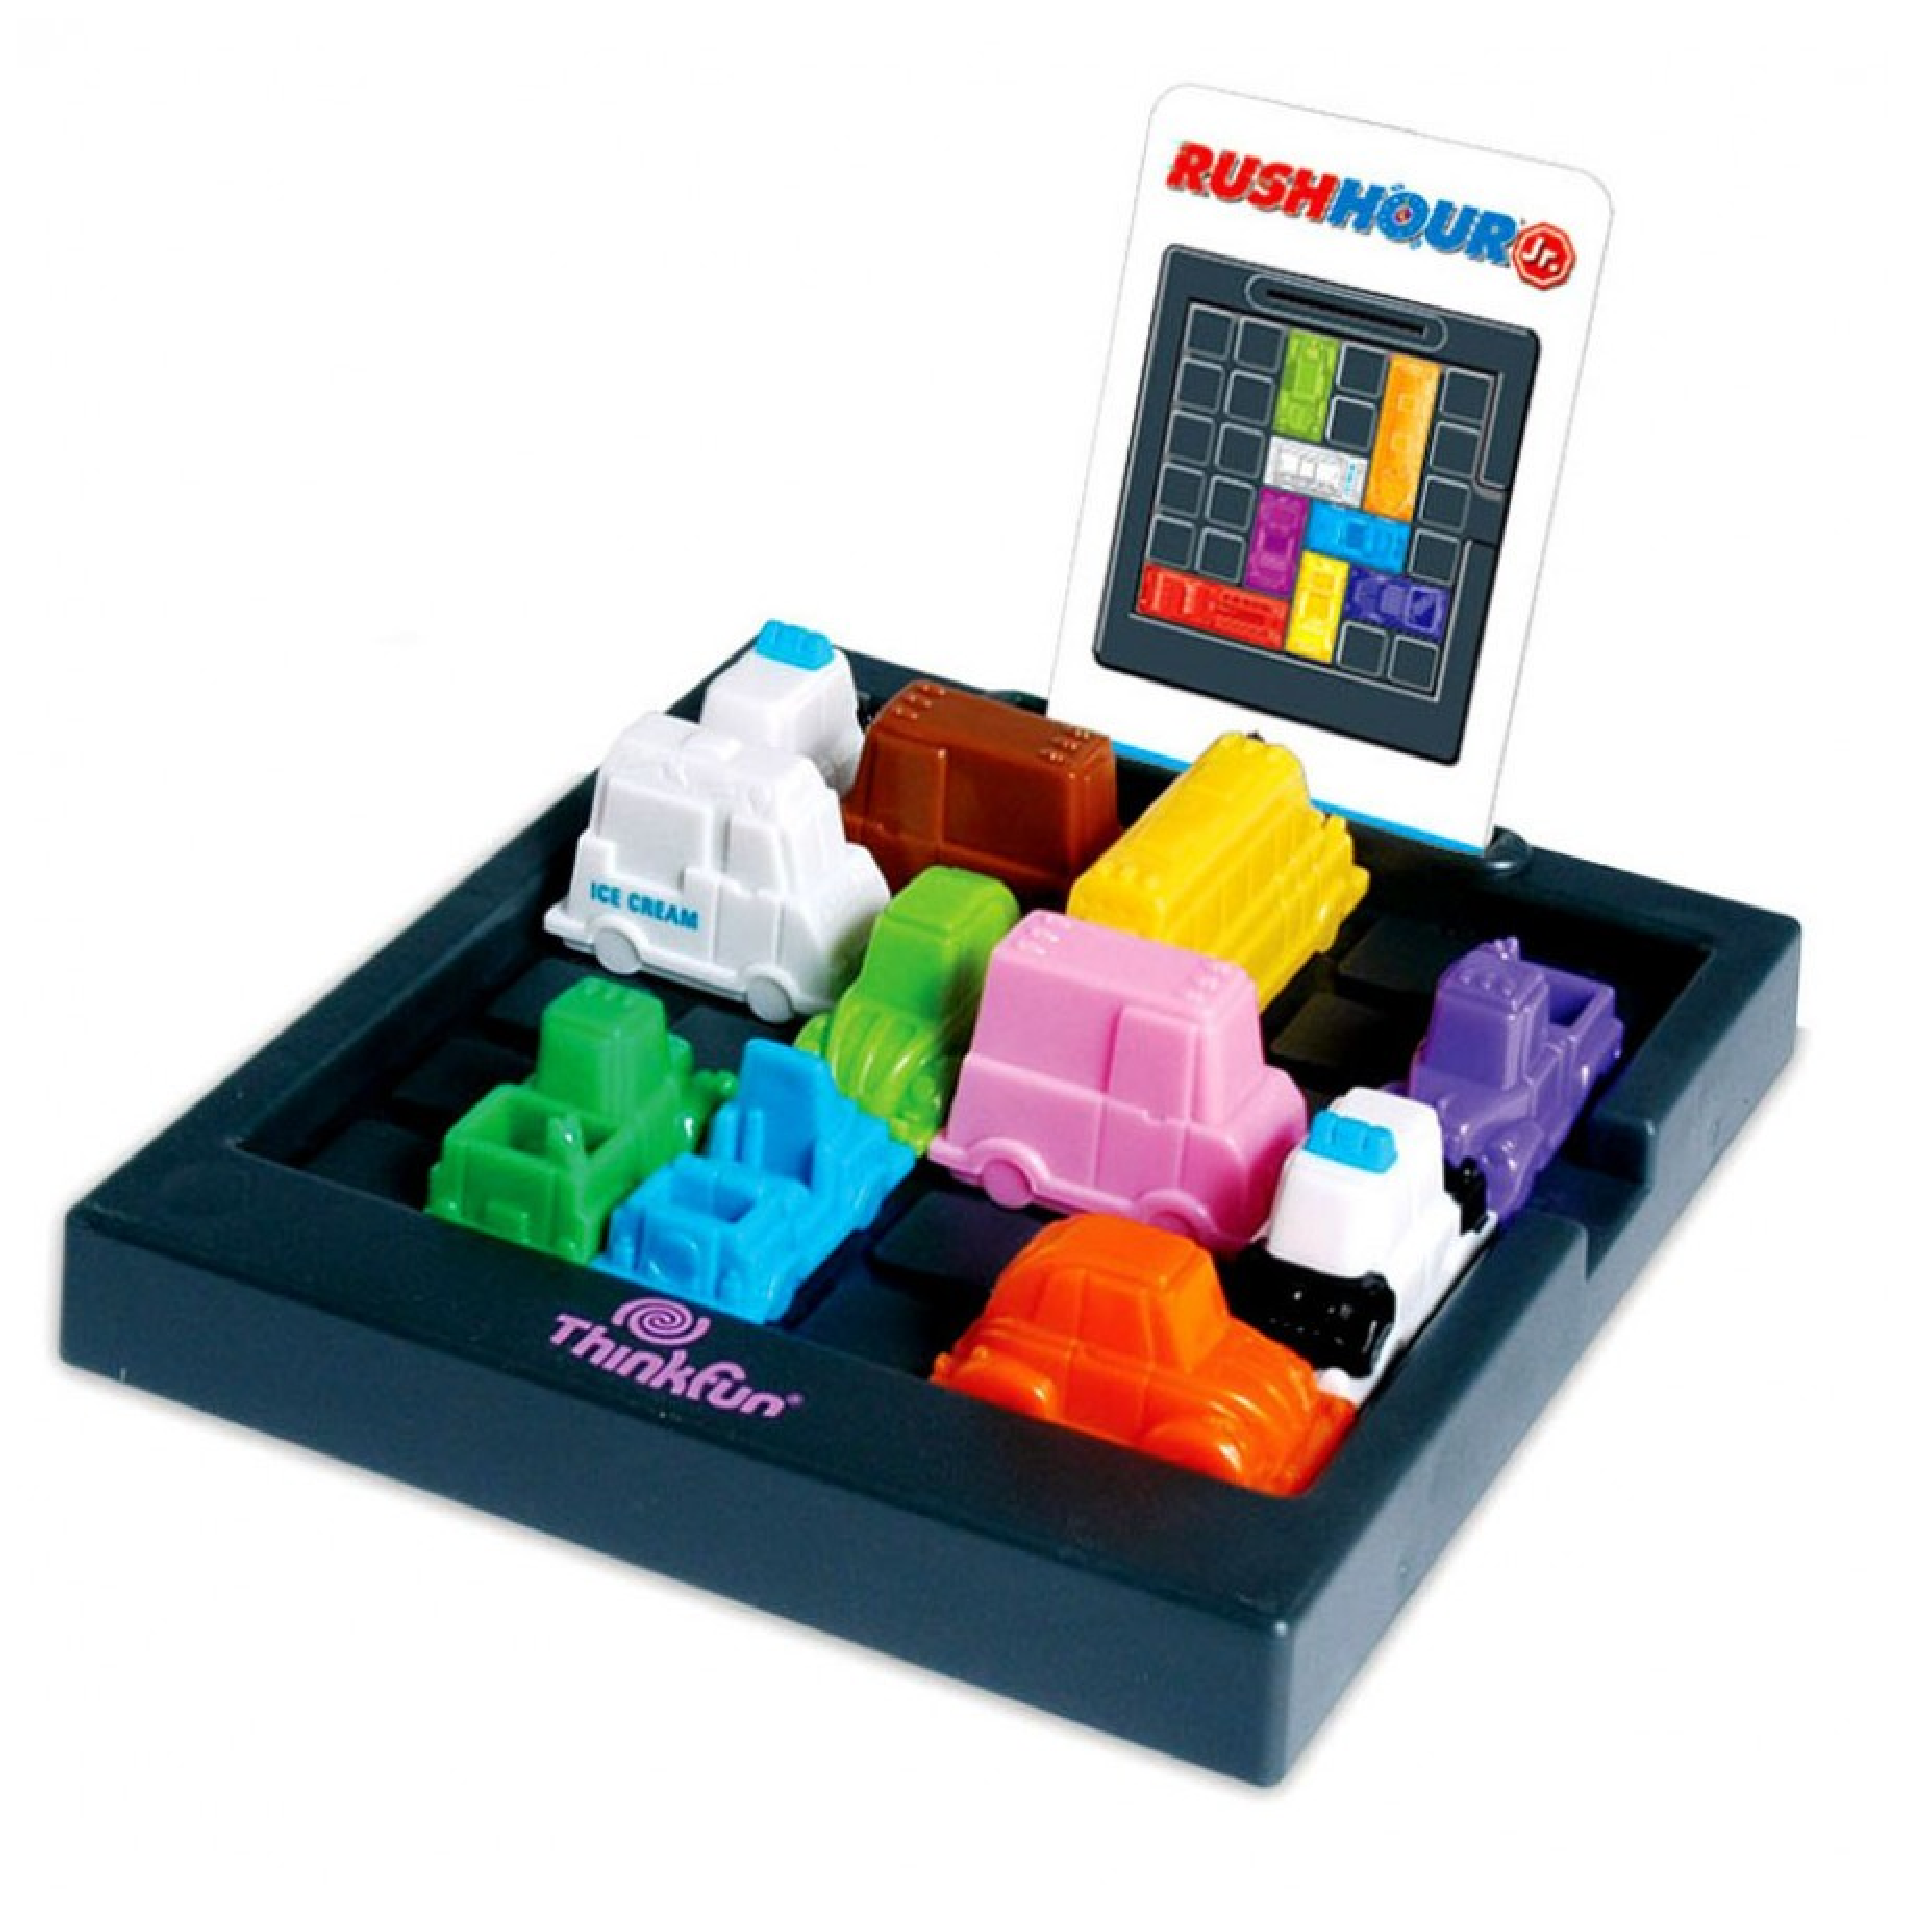
\includegraphics[width=6cm]{Nombres_et_calculs_did/Images/Num2_activites_Rush_hour}
\end{minipage}

{\bf Objectif :} à partir d’un état initial, organiser une suite d’actions pour atteindre un but. C'est un tâche complexe qui nécessite une appropriation. \\

{\bf But du jeu} : faire sortir la voiture rouge de l'aire de stationnement en respectant les règles d'action : avancer ou reculer sur sa ligne ou sa colonne. Il n'est pas possible de tourner ou de passer par dessus un autre véhicule mais tous les véhicules peuvent être déplacés. \\

{\bf Dans les programmes} : outre le travail de résolution de problèmes, cette activité travaille le domaine 5 \og Explorer le monde \fg{} et plus particulièrement l'item \og Représenter l’espace \fg : par l’utilisation et la production de représentations diverses (photos, maquettes, dessins, plans\dots) et également par les échanges langagiers avec leurs camarades et les adultes, les enfants apprennent à restituer leurs déplacements et à en effectuer à partir de consignes orales comprises et mémorisées. Le passage aux représentations planes les amène à commencer à mettre intuitivement en relation des perceptions en trois dimensions et des codages en deux dimensions [\dots] \\

{\bf Compétences travaillées :}
\begin{itemize}
   \item Situer des objets par rapport à soi, entre eux, par rapport à des objets repères.
   \item Orienter et utiliser correctement une feuille de papier, un livre ou un autre support d’écrit, en fonction de consignes, d’un but ou d’un projet précis.
    \item Utiliser des marqueurs spatiaux adaptés (devant, derrière, droite, gauche, dessus, dessous\dots) dans des récits, descriptions ou explications.
   \item Se repérer sur un quadrillage ;
   \item Essayer, tâtonner, être concentré et persévérer pour résoudre un problème ;
   \item Organiser mentalement une suite d'actions pour atteindre un but et être capable de la reproduire plusieurs fois. \\
\end{itemize}

{\bf Matériel :}
\begin{itemize} 
    \item une grille de jeu de 5 $\times$ 5 cases représentant une aire de stationnement dont la sortie est matérialisée à droite ;
    \item les véhicules : des voitures dont une rouge et des camions ;
    \item une série de cartes-problèmes numérotées de 1 à 24 de difficulté graduelle ;
   \item une feuille de route afin de noter sa progression. \\
\end{itemize}

\begin{center}
   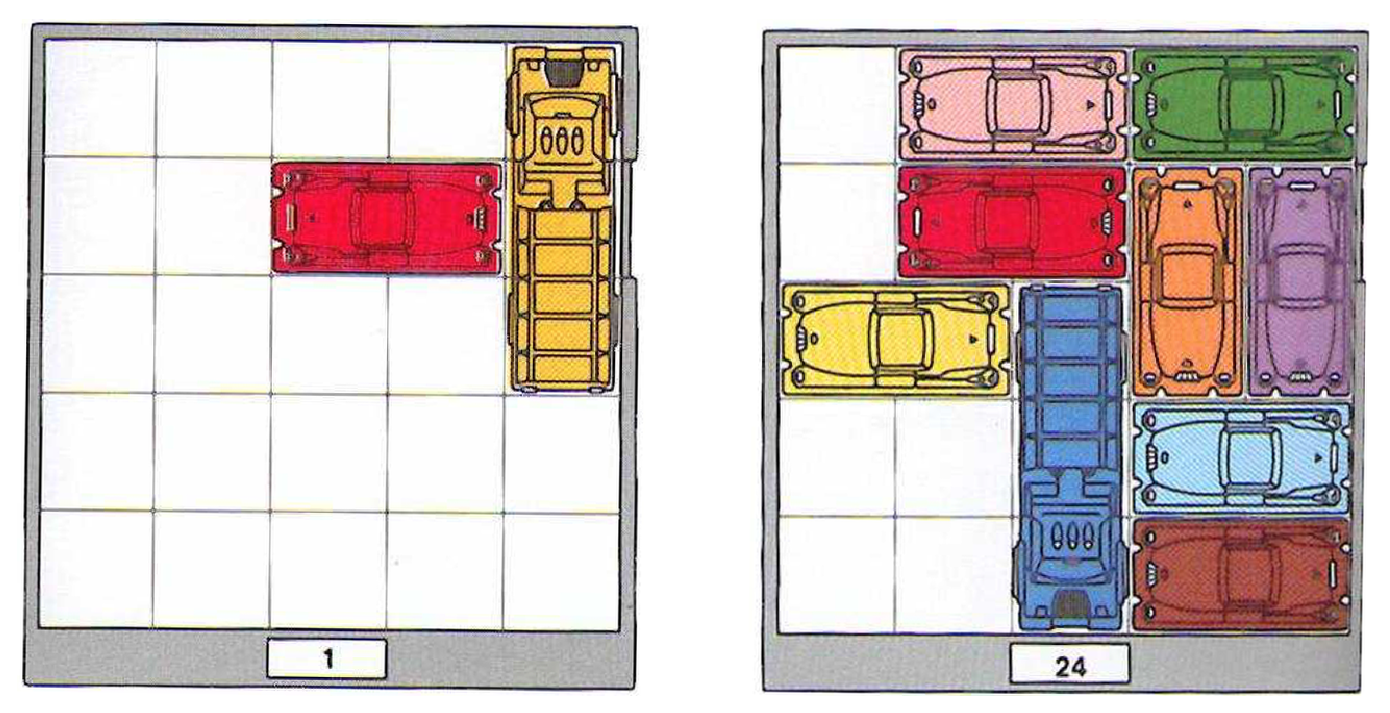
\includegraphics[width=11cm]{Nombres_et_calculs_did/Images/Num2_activites_cartes} \\
   {\it les cartes-problèmes n\degre1 et n\degre24 : l'objectif est de faire sortir la voiture rouge}
\end{center}

{\bf Déroulement de l'activité :}
\begin{description}
  \item[Étape 1 :] {\bf présentation du matériel et des règles de déplacement.} \\
  L'enseignant présente le parking : \og Les véhicules ne peuvent pas être retirés du plateau et ne peuvent qu'avancer ou reculer dans leur couloir sur lequel ils sont placés \fg. L'enseignant donne le but à atteindre : fair sortir la voiture rouge du parking. \\
  Après avoir posé la voiture rouge et quelques autres véhicules sur le parking, on constate que la voiture rouge est bloquée. Il faut cependant la faire sortir du parking. L'enseignant demande à un enfant de faire rouler la voiture rouge et quelques autres véhicules, mais pas de la faire sortir. On ne s'intéresse ici qu'au respect des règles de déplacement.
  \item[Étape 2 :] {\bf appropriation de la situation en petits groupes.} \\
  L'enseignant place sur le plateau du parking les voitures suivant une première configuration. Un enfant est invité à montrer l'endroit de la sortie qui n'est pas très visible lorsqu'un véhicule est placé devant. Puis l'enseignant demande si la voiture peut sortir et ce qu'il faut faire pour qu'elle puisse sortir. Il demande quel véhicule il faut déplacer et de proche en proche il fait déplacer tous les véhicule afin d'arriver à l'objectif.
  \item[Étape 3 :] {\bf résolution des problèmes.} \\
  Cette phase est proposée à tous les enfants qui ont pu s'approprier l'ensemble de la situation dans l'étape précédente. Elle ne commence donc pas forcément au même moment pour tous les enfants. Chaque enfant prend sa feuille de route et coche les problèmes numérotés qu'il a résolus. Le contrat est exposé aux enfants soit au cours d'un regroupement, soit de manière individuelle :
  \begin{itemize}
     \item tu prends une carte-problème numérotée ;
     \item tu disposes les voitures comme sur la carte-problème (GS) ou tu me demande de les poser (PS-MS) ;
     \item tu essaies de faire sortir la voiture rouge ;
     \item quand tu as réussi à la faire sortir, tu remets les voitures à la même place qu'au début et tu recommences pour être sûr de la façon de la faire sortir ;
     \item si tu y arrives une seconde fois, tu peux mettre une croix dans la case de ta feuille de route ;
     \item un peu plus tard, tu me montreras à nouveau comment tu as fait. \\
  \end{itemize}
\end{description}

{\bf Une version numérique :} la version adaptée du jeu de société est disponible sur Internet. \href{https://micetf.fr/embouteillages/}{\it\blue Le jeu à l'identique} peut être utilisé en classe avec un petit groupe d'élèves par exemple.
\end{exercice*}

\pagebreak


\begin{exercice*}[\fbox{C1} - Rituel : la tour d'appel] %%% 1 %%%
   \begin{description}
      \item[Compétences visées] : quantifier des collections jusqu'à 10 dix au moins, les composer, les décomposer par manipulation ; comparer des quantités.
      \item[Objectif] : représenter un petit groupe d'élèves (présents, filles, garçons, MS, GS\dots) par une tour en briquettes puis la comparer à un modèle. Travailler le vocabulaire \og plus que \fg,  \og moins que \fg, \og autant que \fg{} et le dénombrement.
      \item[Déroulement] :
         \begin{enumerate}
            \item Construire la tour modèle avec les enfants. \\
            Difficulté : pour certains, la modélisation est compliquée. Une briquettes, c’est un enfant. Ne pas hésiter à réaliser cette tour plusieurs fois, le temps que les élèves comprennent cette modélisation. Il est possible d'ajouter une étiquette photo ou prénom sur les briquettes dans un premier temps.
            \item Les enfants construisent la tour du jour. À l’arrivée en classe, en même temps que l’enfant va chercher son étiquette prénom, il prend une briquettes dans une barquette pour l’ajouter à la tour du jour. \\
            Dans la barquette, il doit y avoir autant de briquettes que d’enfants inscrits, cela permet de valider en faisant le lien avec les étiquettes des absents.
            \item La tour du jour est réalisée par un seul enfant pendant l’appel en s’appuyant sur les tableaux présents/absents. Il la présente à ses camarades pendant le regroupement.
         \end{enumerate}
      \item[Variantes] : compter les présents, dire combien il faut ajouter d'élèves pour obtenir tous les élèves de la classe ; travailler les décompositions des nombres, avec ou sans couleurs ; construire une tour par jour et les comparer en fin de semaine.
      \item[Exemples] : \href{https://www.youtube.com/watch?v=1W5twrzjv5I}{\it\blue La tour d'appel en moyenne section}. \href{https://www.youtube.com/watch?v=7quHGbemeiM&t=61s}{\it\blue La tour d'appel en grande section}.
   \end{description}
   \begin{center}
   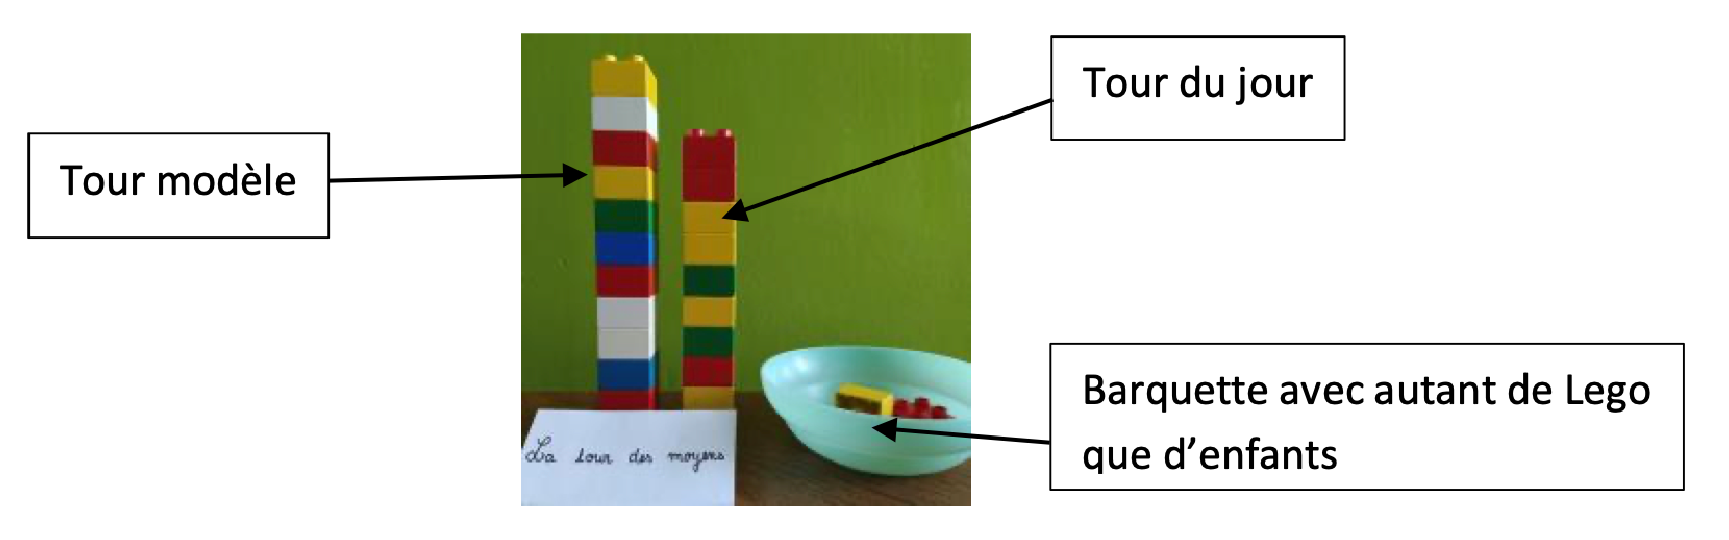
\includegraphics[width=12cm]{Nombres_et_calculs_did/Images/Num2_activites_tour_appel}
\end{center}
\end{exercice*}


\begin{exercice*}[\fbox{C2} - Des jeux pour travailler les tables de multiplication]
\begin{tabular}{p{8cm}|p{8cm}}
   {\bf Le domino des multiplications} \newline
   \href{http://www.charivarialecole.fr/2016/10/27/a3427665/}{\it\blue Lien vers le site \og Charivari \fg.} 
   \begin{center}
      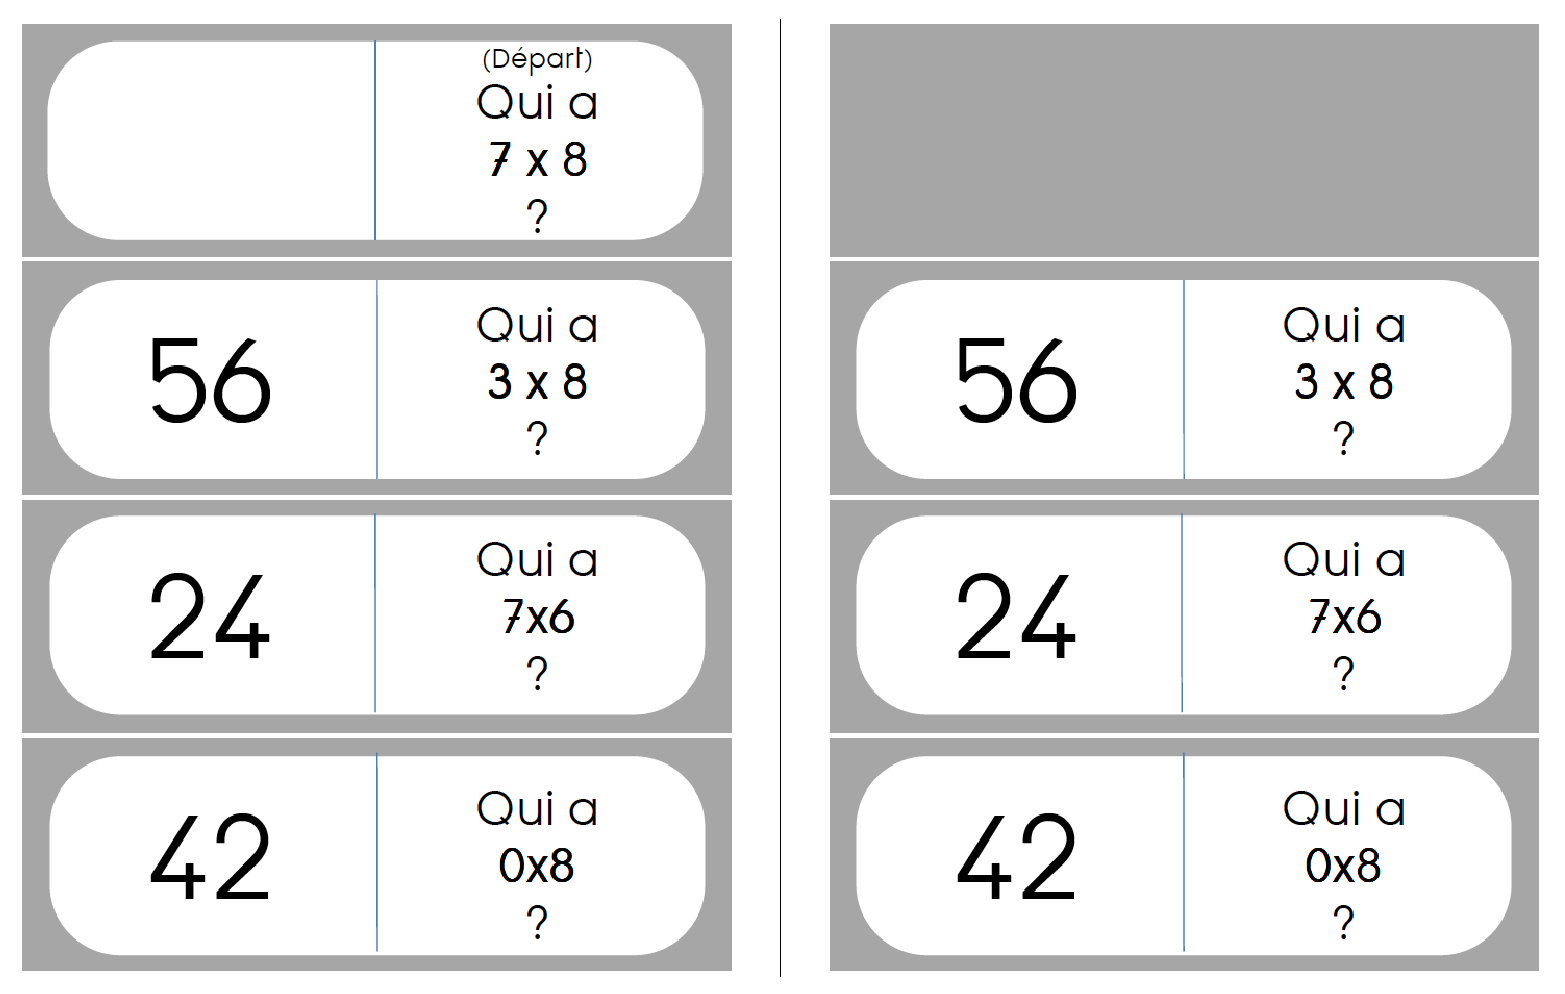
\includegraphics[height=4cm]{Nombres_et_calculs_did/Images/Num2_activites_dominos}
   \end{center}
   &
   {\bf Les cocottes des multiplications} \newline
   \href{https://lutinbazar.fr/wp-content/uploads/2015/04/cocotte-tables-multiplication-LB.pdf}{\it\blue Lien vers le site de \og Lutinbazar \fg} 
    \begin{center}
      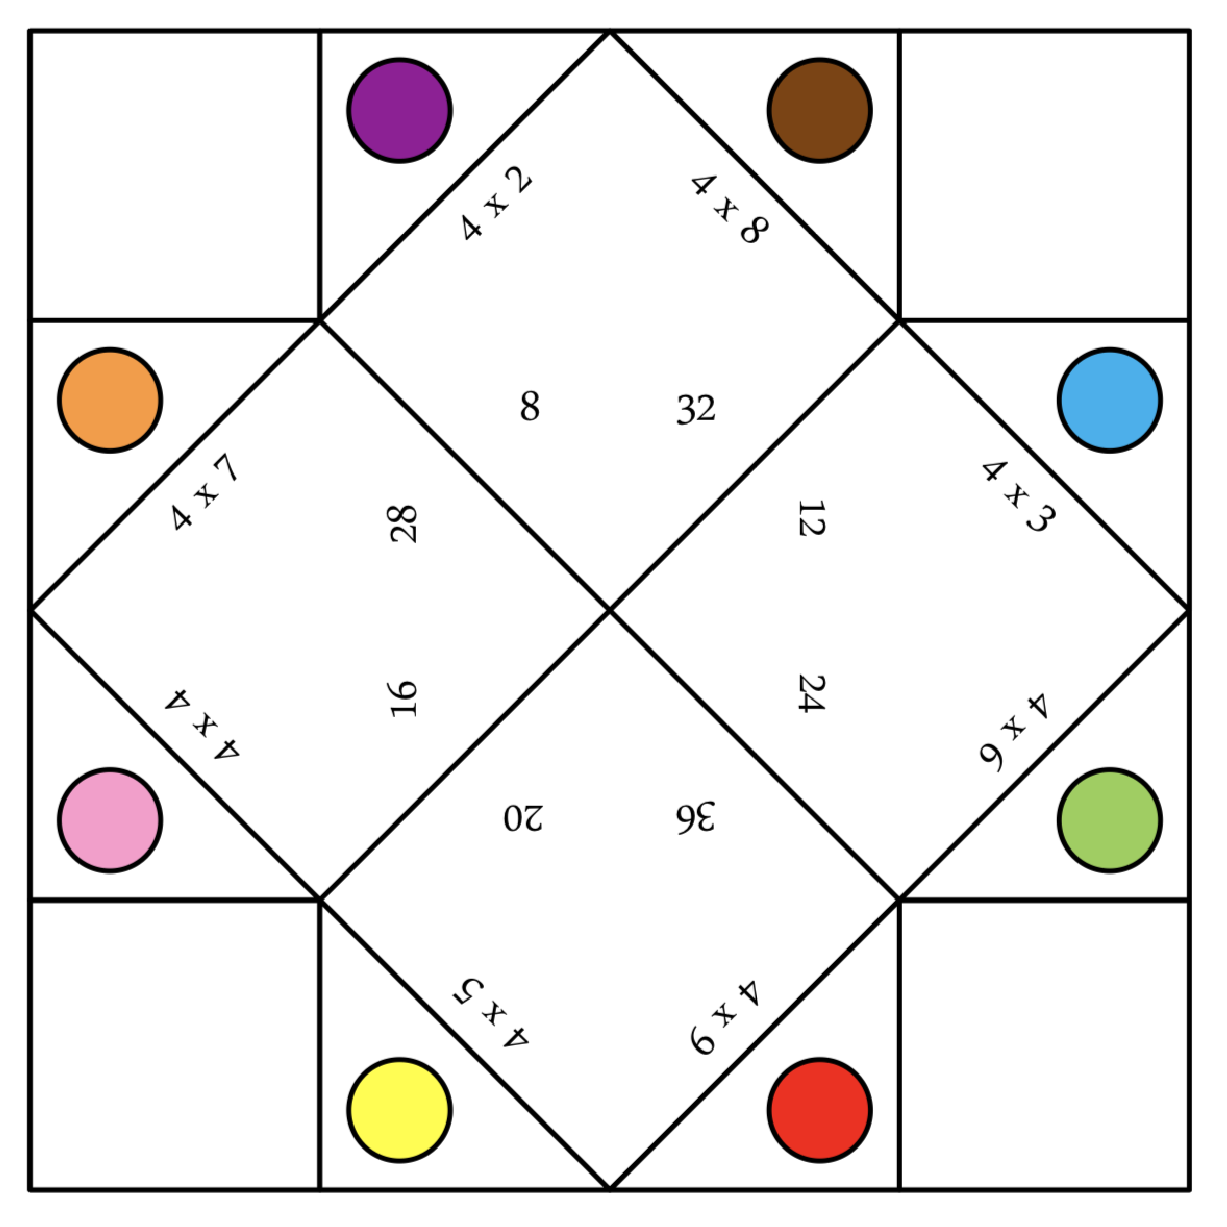
\includegraphics[height=4cm]{Nombres_et_calculs_did/Images/Num2_activites_cocote}
   \end{center}
   \\ [-5mm] 
   {\bf Connaissances travaillées} : connaître des tables de multiplication.
   &
   {\bf Connaissances travaillées} : connaître ses tables de multiplication. \\
   {\bf Principe du jeu :} jeu des dominos.
   &
   {\bf Principe du jeu :} jeu de la cocotte. \\
\end{tabular}
%%%
\end{exercice*}


\begin{exercice*}[\fbox{C2/C3} - Fiches de résolution de problèmes classiques] %%%
Des exemples d'activités de résolution de problèmes foisonnent dans les manuels et sur la toile, par exemples :
\begin{itemize}
   \item pour la maternelle, des cartes de problèmes de \href{http://lamaitresseaupetitpois.eklablog.com/des-problemes-mathematiques-en-maternelle-a157565476}{\it\blue La maîtresse au petit pois} ;
   \item pour le CE1, des fiches du blog \href{https://classeurdecole.wordpress.com/2012/02/07/resolution-de-problemes-ce1-2/}{\it\blue Classeur d'école} classées par thèmes : résoudre un problème additif, rechercher une différence, rechercher la condition initiale, résoudre un problème avec des euros\dots ;
   \item pour le CE2 et le CM1, des fiches pour le cycle 3 (programmes de 2008) classées par compétence à développer : appliquer des consignes, reconnaître un problème, identifier la consigne, associer une question à un problème, repérer les données utiles, reconstituer un énoncé\dots
   \item des fiches de défis maths ou rallyes maths proposées dans de nombreuses académies. L'intérêt est de faire des mathématiques une source de plaisir, de valoriser le travail en équipe, d'inciter au débat mathématique, de favoriser l'autonomie des élèves, de développer certaines stratégies d'apprentissages\dots
\end{itemize}
\end{exercice*}

\bigskip

\begin{exercice*}[\fbox{C2/C3} - Le concours kangourou] %%%
   Le \href{http://www.mathkang.org/concours/}{\it\blue concours kangourou} est un jeu de mathématiques créé en 1991 sur le modèle du concours national australien (d'où son nom). Il comporte 24 questions à choix multiple de difficulté croissante, proposées le même jour dans tous les établissements scolaires du CE2 aux classes supérieures. La liste des sujets est disponible dur le site \href{http://www.mathkang.org/concours/}{\it\blue Le kangourou des mathématiques}, ils sont tous corrigés et peuvent être utilisés en classe librement. \\
   Il est possible de faire effecteur aux élèves entièrement un sujet (le temps théorique est de 50 minutes), mais on peut également se servir des sujets pour créer des fiches de mini résolutions de problèmes, à utiliser en autonomie par exemple lorsqu'un élève a terminé son travail. Un avantage est que ces sujets est qu'ils balayent tous les domaines abordés à l'école par le biais de questions logiques.
    \begin{center}
      \fbox{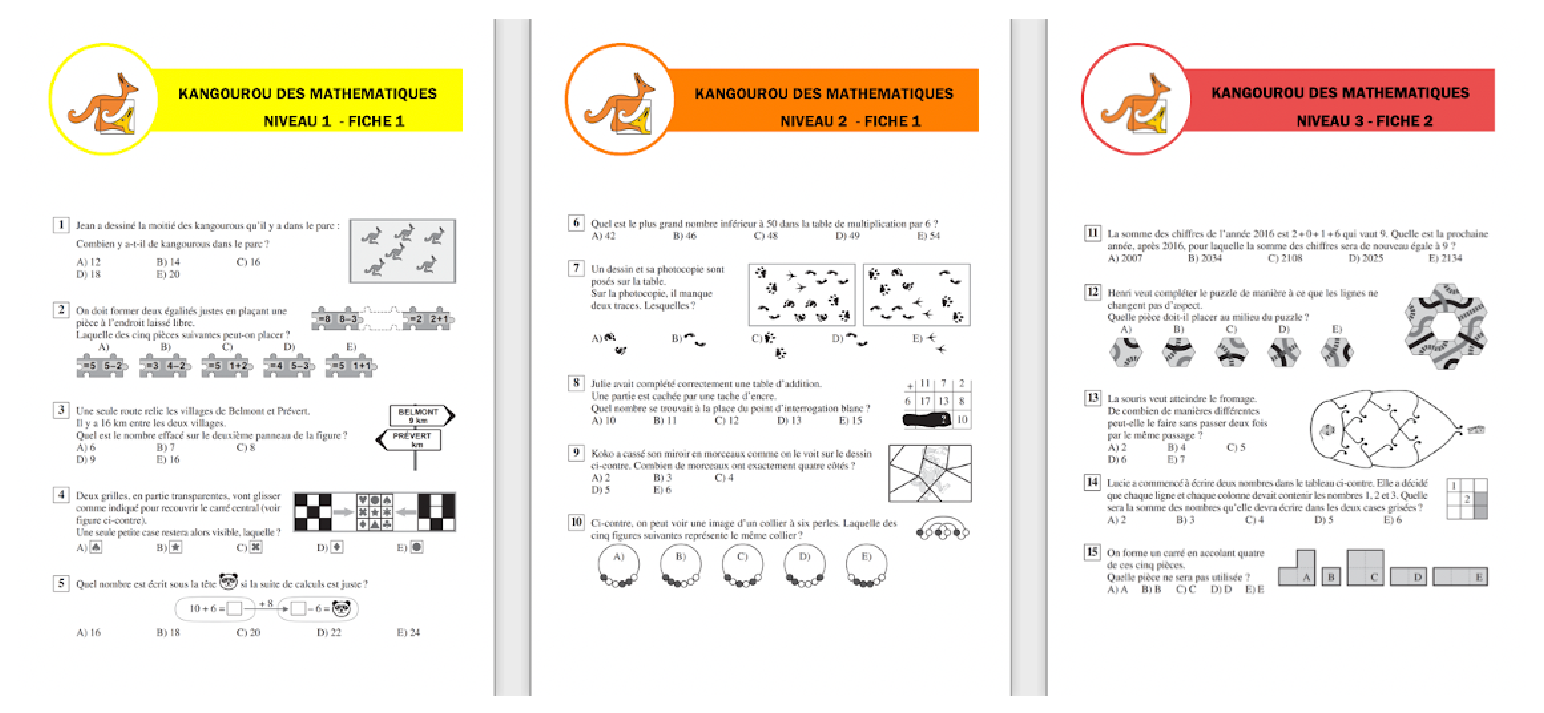
\includegraphics[width=17cm]{Nombres_et_calculs_did/Images/Num2_activites_kangourou}}
   \end{center}
   Les questions sont graduées : les 8 premières sont les plus simples, les 8 suivantes un peu plus complexes et les 8 dernières encore plus compliquées. \\
   Le document présenté est constituées de fiches de cinq questions. Avec un sujet de concours, quatre fiches (de 1 à 4) de niveau de plus en plus ardu sont proposées, jusqu'à la question 20 mais on peut tout à fait envisager une autre configuration !
\end{exercice*}

